\documentclass[slidestop,compress,mathserif, aspectratio = 169]{beamer}
\usetheme[block = fill, numbering = none]{metropolis}
\usepackage{etex}
\useinnertheme{rectangles}
\usepackage{graphicx}
\usepackage{subfig}
\usepackage{epigraph}
\usepackage{makeidx}
\usepackage[]{amsmath}
\usepackage[]{amssymb}
\usepackage{color}
\usepackage{pict2e}
\usepackage{algorithm2e}
\usepackage[english]{babel}
\usepackage{tikz}
\usetikzlibrary{mindmap}
\usepackage{multirow}
\usepackage{ulem}
\usepackage[utf8]{inputenc}
\usepackage{multimedia}
\usepackage{xcolor}
\usepackage{keyval}
\usepgfmodule{shapes}
\usepackage{pgfplots}
\usepackage{sansmath}
\usepackage{pgfgantt}
\usetikzlibrary{arrows}
\usetikzlibrary{graphs, automata, spy, positioning}
\usetikzlibrary{shapes.gates.logic.US,trees}
\usepackage{colortbl}
\usepackage{array}
\usepackage{listings}
\usepackage{pdfpages}
\usepackage{textcomp}
\pgfplotsset{width=6cm}


%\definecolor{RYB1}{RGB}{240,249,232}
%\definecolor{RYB2}{RGB}{186,228,188}
%\definecolor{RYB3}{RGB}{123,204,196}
%\definecolor{RYB4}{RGB}{67,162,202}
%\definecolor{RYB5}{RGB}{18,104,172}
%
%\definecolor{blue}{rgb}{0,0,1}
%\definecolor{mint}{cmyk}{75,0,40,0}
%\definecolor{mint}{rgb}{32,178,170}
\graphicspath{{./AIMethods/figures/}}

\AtBeginSection{\frame{\sectionpage}}
%\AtBeginSubsection{\frame{\subsectionpage}}
\newtranslation[to=ngerman]{Section}{Teil}
\newtranslation[to=ngerman]{Subsection}{Abschnitt}

\setbeamersize{text margin left=.8cm, text margin right=.8cm}

%\setbeamertemplate{frametitle}{%
%    \nointerlineskip%
%    \begin{beamercolorbox}[wd=\paperwidth,ht=2.0ex,dp=0.6ex]{frametitle}
%        \hspace*{1ex}\insertframetitle%
%    \end{beamercolorbox}%
%}

\newcommand\MyBox[2]{
  \fbox{\lower0.75cm
    \vbox to 1.7cm{\vfil
      \hbox to 1.7cm{\hfil\parbox{1.4cm}{#1\\#2}\hfil}
      \vfil}%
  }%
}

\pgfmathdeclarefunction{norm}{3}{%
                      \pgfmathparse{sqrt(0.5*#3/pi)*exp(-0.5*#3*(#1-#2)^2)}%
                    }
\begin{document}

\setbeamertemplate{bibliography item}{\insertbiblabel}
\tikzstyle{element} = [draw,rectangle, align = center, text width = 2.5 cm, node distance = 1.25 cm]

% Formalia
\newcommand{\Var}{\operatorname{Var}}
\newcommand{\mum}{\operatorname{\mu m}}
\newcommand{\E}{\operatorname{E}}
\newcommand{
\offslide}[2]{
\begin{frame}
\frametitle{\includegraphics[scale=0.05] {Offwhite} \hspace{.5mm} #1}
%\framesubtitle{#2}
\begin{tikzpicture}[x=1cm, y=1cm, semitransparent]
\draw[step=5mm, line width=0.2mm, black!40!white] (0,0) grid (\textwidth,\textheight-1cm);
\node[anchor = south east] at (\textwidth,0) {#2};

\end{tikzpicture}
\end{frame}
}
\newcommand{\source}[1]{\rotatebox{90}{\tiny \color{gray} #1}}

\newcommand{\lehrtext}[1]{
\only<article>{
\vspace{0.3cm}
\leavevmode%
  \tabto*{-1.8cm}% LEFT MARGIN
  %\tabto*{\dimexpr\linewidth+40pt\relax}% RIGHT MARGIN
  \smash{\belowbaseline[-\ht\strutbox]{\makebox[0pt]%
%    [r]% LEFT MARGIN
    [l]% RIGHT MARGIN
  {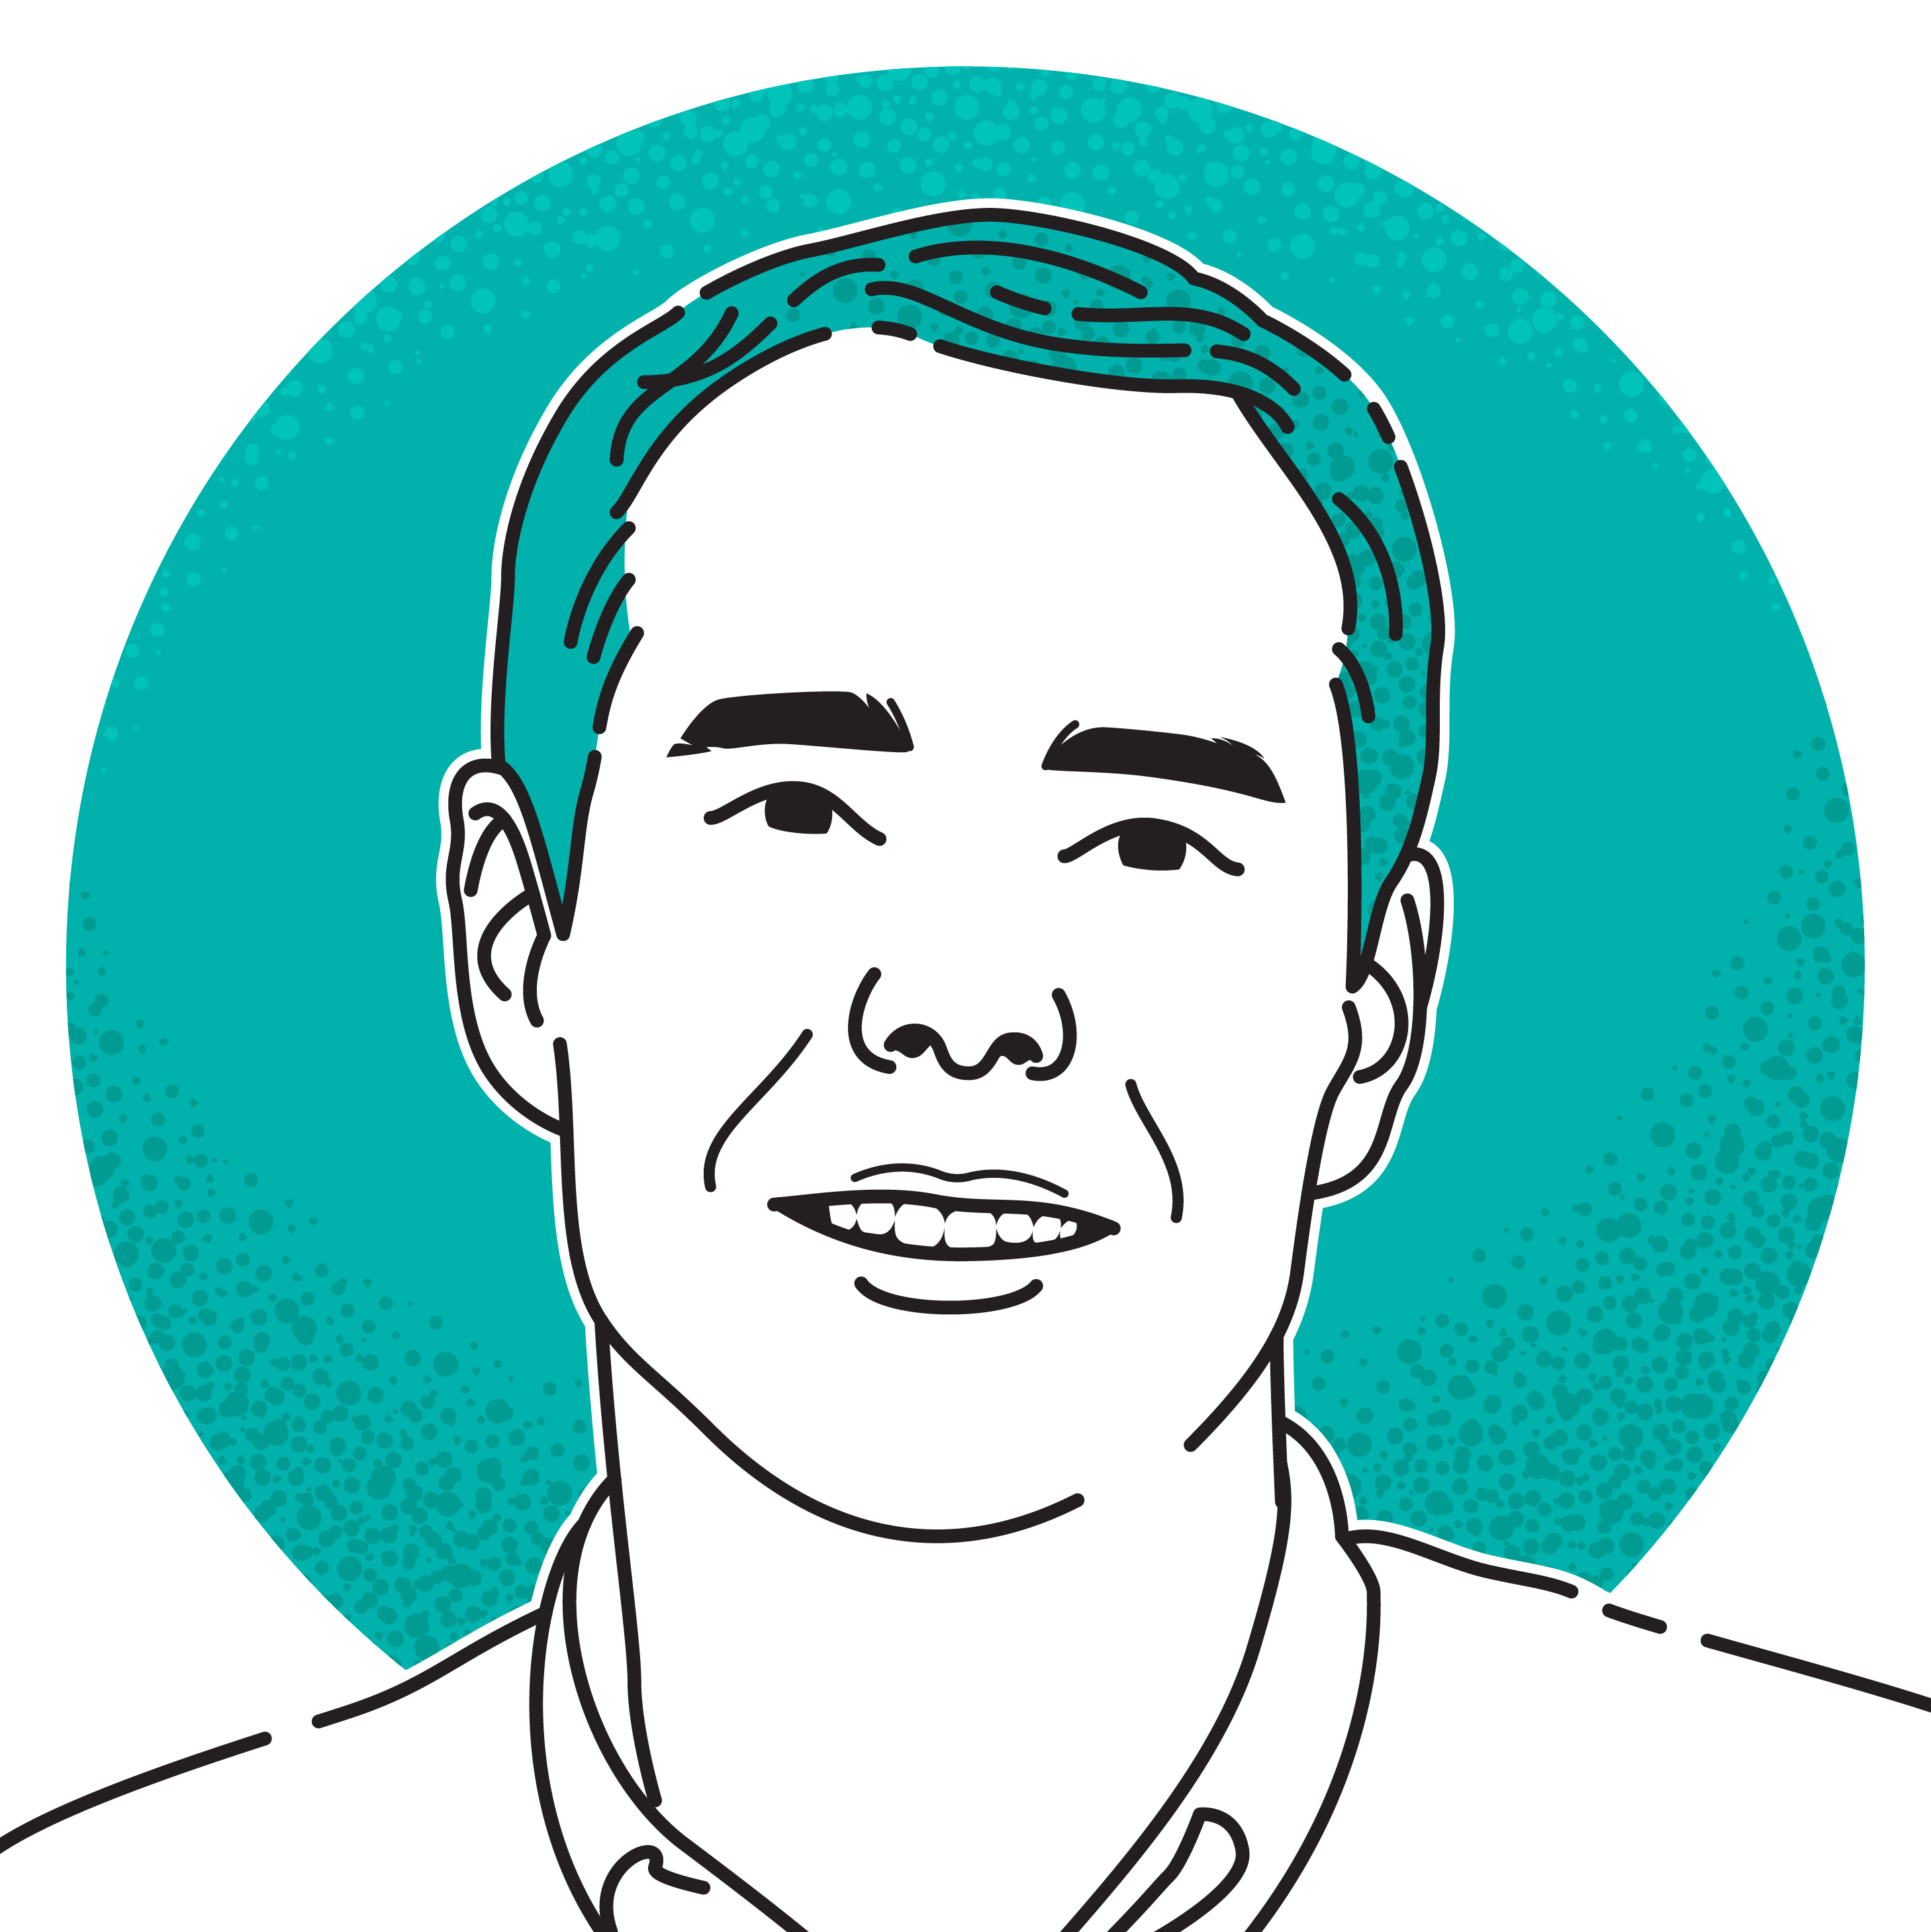
\includegraphics[width = 1.5cm]{teacher}}}}%
  \tabto*{\TabPrevPos}%
#1
}
}

\title{Rail Data Science}
\subtitle{AI Methods}
\author{Prof. Dr. Raphael Pfaff}
\institute[FH Aachen]{Fachhochschule Aachen}
\logo{\put(-18, 120){
\includegraphics[width=1.4cm]{logoR}}}

\begin{frame} % Cover slide
\titlepage
\end{frame}

% !TEX root = ../ifvWorkshopQuality.tex

\frame{\frametitle{What is machine learning?}
\framesubtitle{ML is a field of study that gives computers the ability to learn without being explicitly programmed.}
\begin{columns}[t] 
     \begin{column}[T]{7cm} 
     	\begin{itemize}
     		\item Different paradigm:
		\begin{itemize}
		\item Derive rules from observations
		\end{itemize}
		\item Typical procedure:
		\begin{itemize}
		\item \textbf{Train:} Observe set of examples ``training data''
		\item \textbf{Fit:} Infer information of process behind data
		\item \textbf{Test:} Make prediction on unseen data ``Test data''
		\end{itemize}
		\item Variations:
		\begin{itemize}
		\item Supervised learning: provide labels with data
		\item Unsupervised learning: cluster data based on patterns
		\end{itemize}
     	\end{itemize}
     \end{column}
     	\begin{column}[T]{7cm} 
         	\begin{center}
			Traditional approach:
			\vspace{.5cm}
			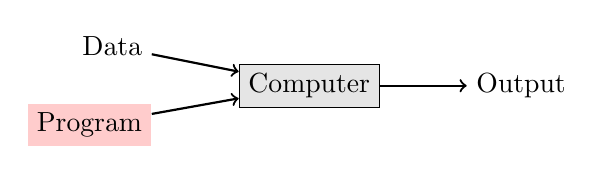
\begin{tikzpicture}
 				\node[anchor = east] (d) at (0,0) {Data};
				\node[anchor = east, fill = red!20] (p) at (0,-1) {Program};
				\node[anchor = west] (o) at (4,-.5) {Output};
				\node[draw, fill = gray!20] (c) at (2,-.5) {Computer};
				\draw[->, thick] (d) -- (c);
				\draw[->, thick] (p)-- (c);
				\draw[->, thick] (c) -- (o);
			\end{tikzpicture}
			
			Machine learning approach:
			\vspace{.5cm}
			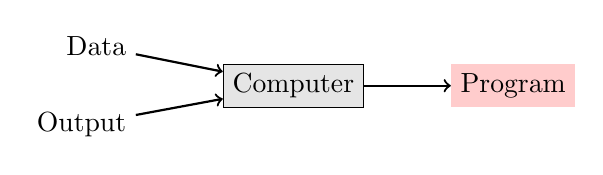
\begin{tikzpicture}
 				\node[anchor = east] (d) at (0,0) {Data};
				\node[anchor = east] (p) at (0,-1) {Output};
				\node[anchor = west,  fill = red!20] (o) at (4,-.5) {Program};
				\node[draw, fill = gray!20] (c) at (2,-.5) {Computer};
				\draw[->, thick] (d) -- (c);
				\draw[->, thick] (p)-- (c);
				\draw[->, thick] (c) -- (o);
			\end{tikzpicture}

		\end{center}
     \end{column}
 \end{columns}
}

\subsection{Unsupervised Learning (Clustering)}
%\frame{\frametitle{Machine Learning}
%\framesubtitle{Using MIT OpenCourseware Slides}
%Source:
%\begin{center}
%Eric Grimson, John Guttag, and Ana Bell. 6.0002 Introduction to Computational Thinking and Data Science. Fall 2016. Massachusetts Institute of Technology: MIT OpenCourseWare, https://ocw.mit.edu. License: Creative Commons BY-NC-SA.
%\end{center}
%}
%\setbeamercolor{background canvas}{bg=}
%%\frame{
%\includepdf[page = 4-6]{OCW/ML.pdf}%}

\frame{\frametitle{Clustering}
\framesubtitle{Two fundamental approaches, $k$ number of clusters defined \textit{a priori}}
\begin{columns}[t] 
     \begin{column}[T]{7cm} 
     \textbf{Hierarchical clustering}
     	\begin{enumerate}
     		\item Assign each item to one cluster
		\item Find closest (most similar cluster): merge them
		\item Continue until desired number of clusters $k$ is reached
     	\end{enumerate}
     \end{column}
     	\begin{column}[T]{7cm} 
         	\textbf{K-means clustering}
     	\begin{enumerate}
		\item Randomly choose $k$ initial centroids
		\item While centroids don't change
		\begin{enumerate}
		\item[E:] Create $k$ clusters by assigning each item to closest centroid
		\item[M:] Compute $k$ new centroids by averaging items in each cluster
		\end{enumerate}
     	\end{enumerate}
     \end{column}
 \end{columns}
 
\begin{center}
 	\includegraphics[width = .9\textwidth]{expectation-maximization}
\end{center}
}

\frame{\frametitle{K-means clustering procedure}
         	\begin{center}
            		\only<1>{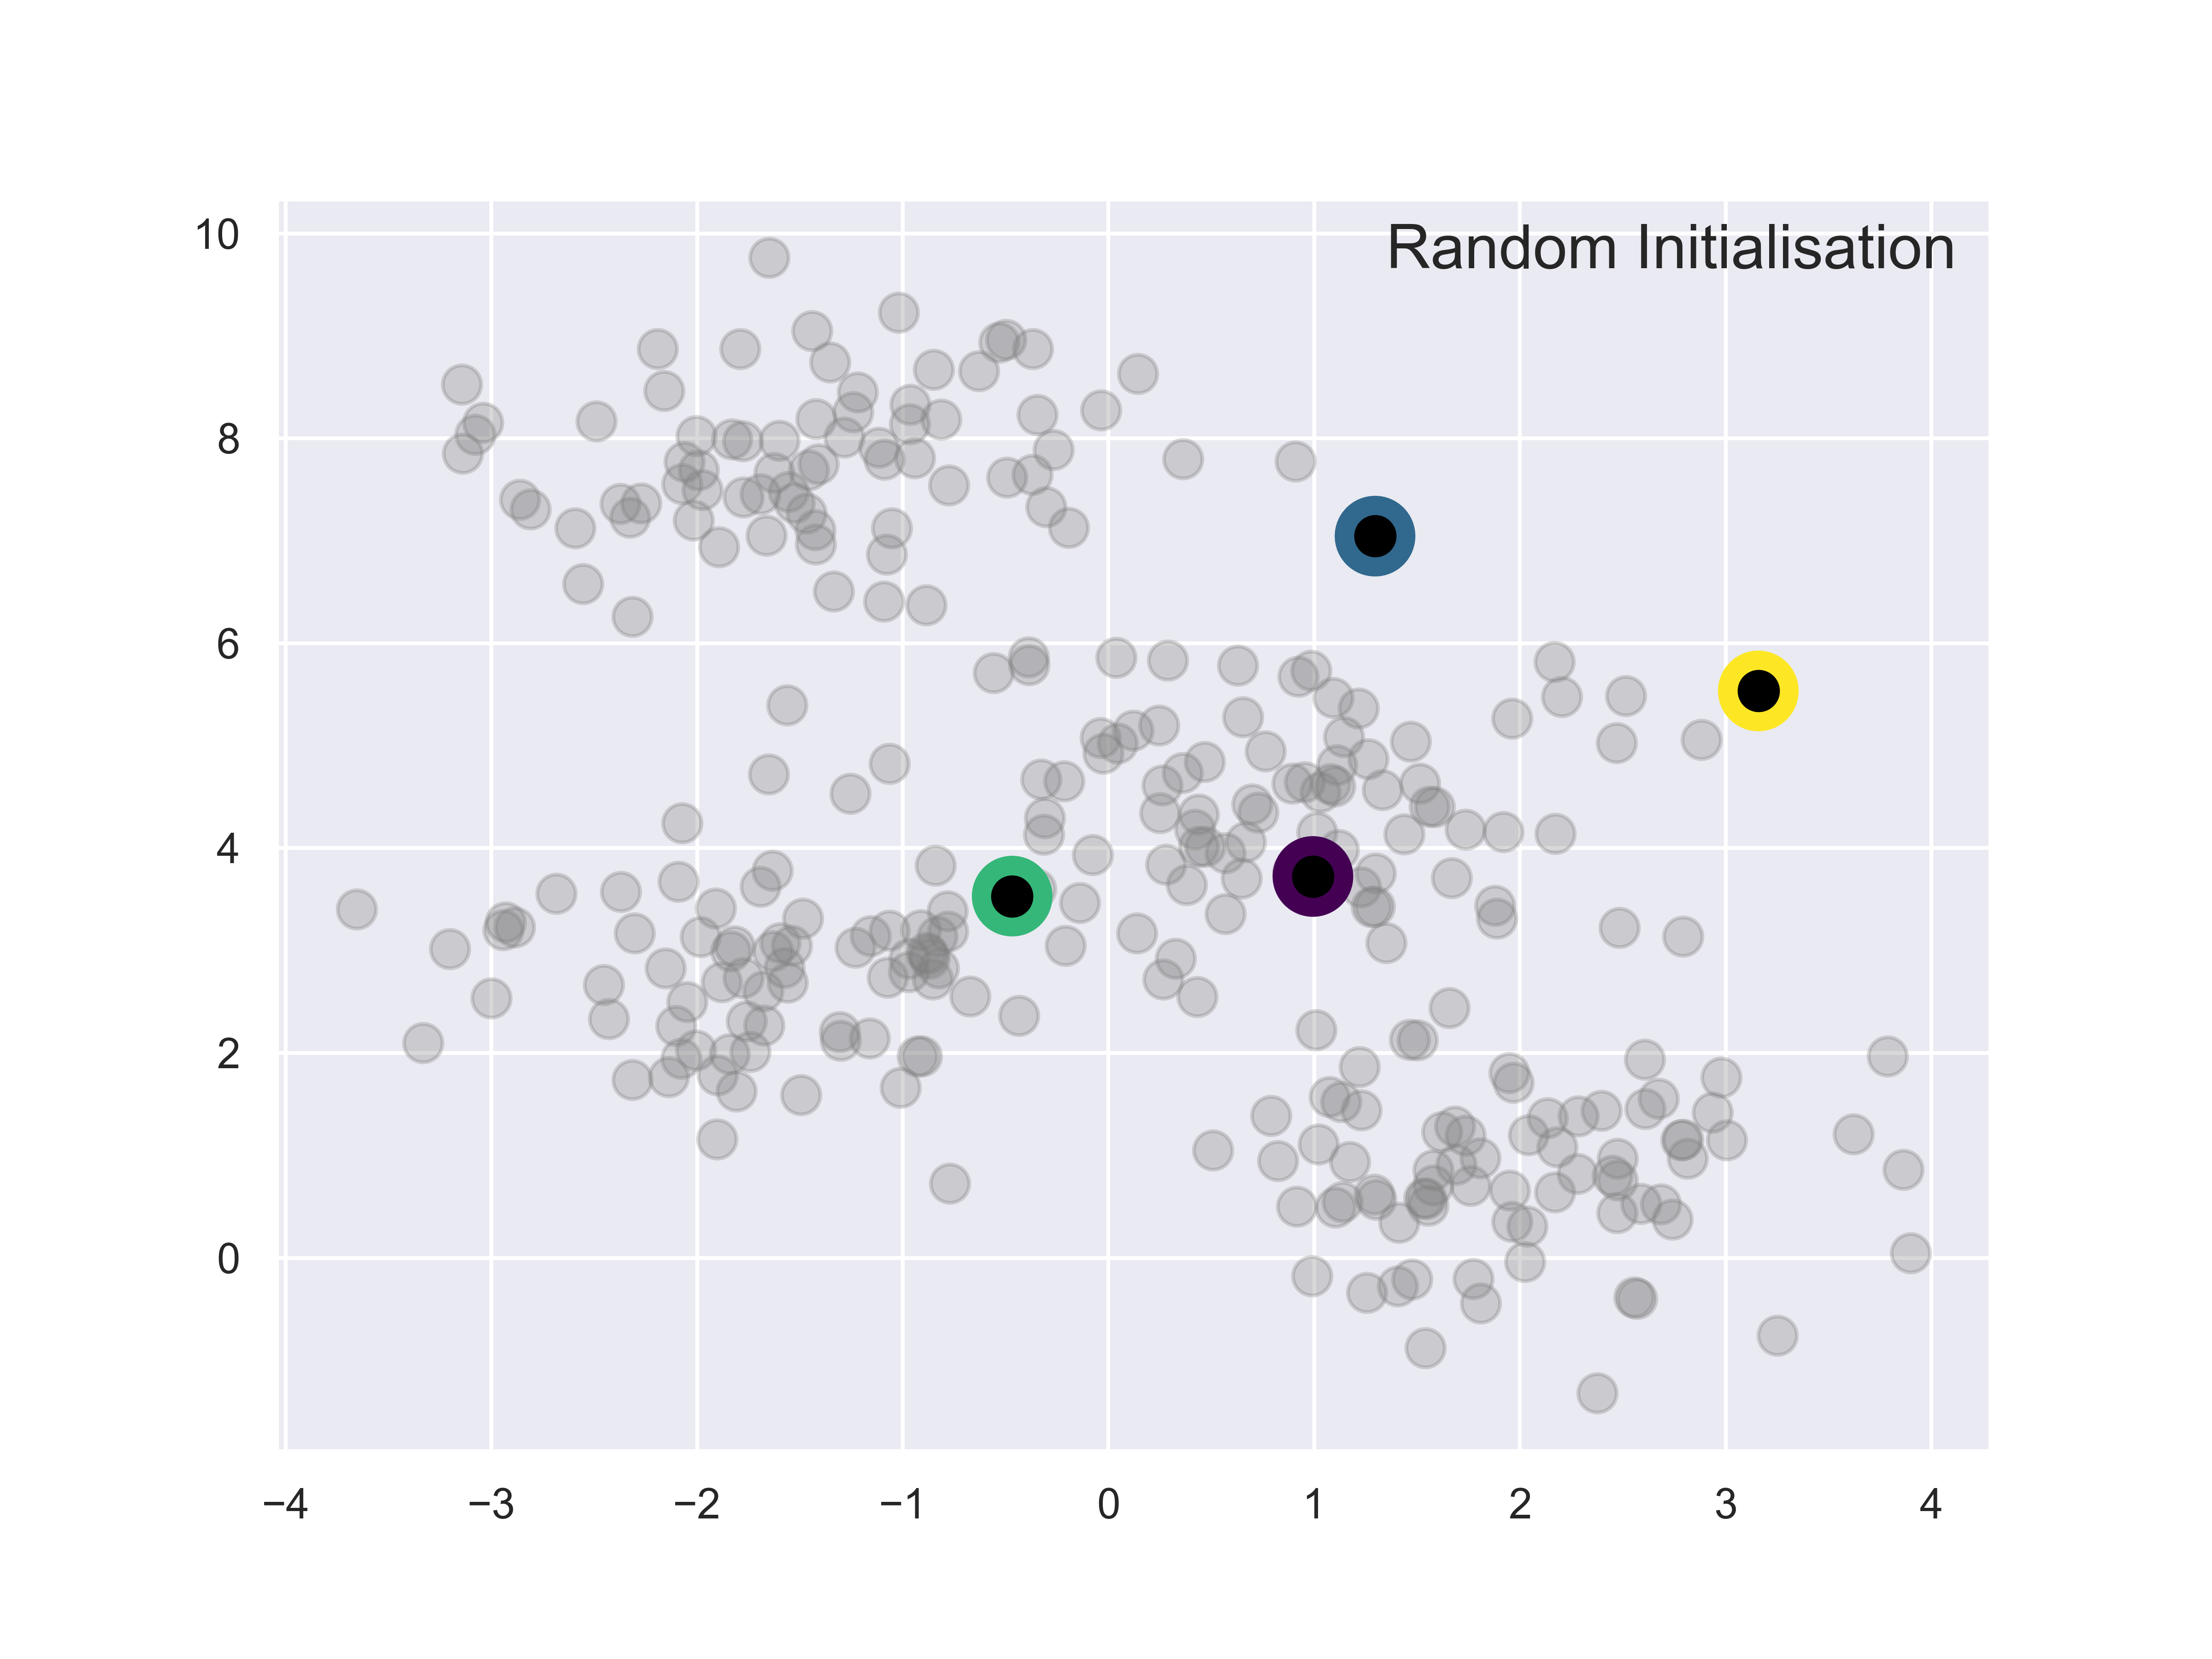
\includegraphics[width=0.7\textwidth]{PCAprocedure0}\source{}}
			\only<2>{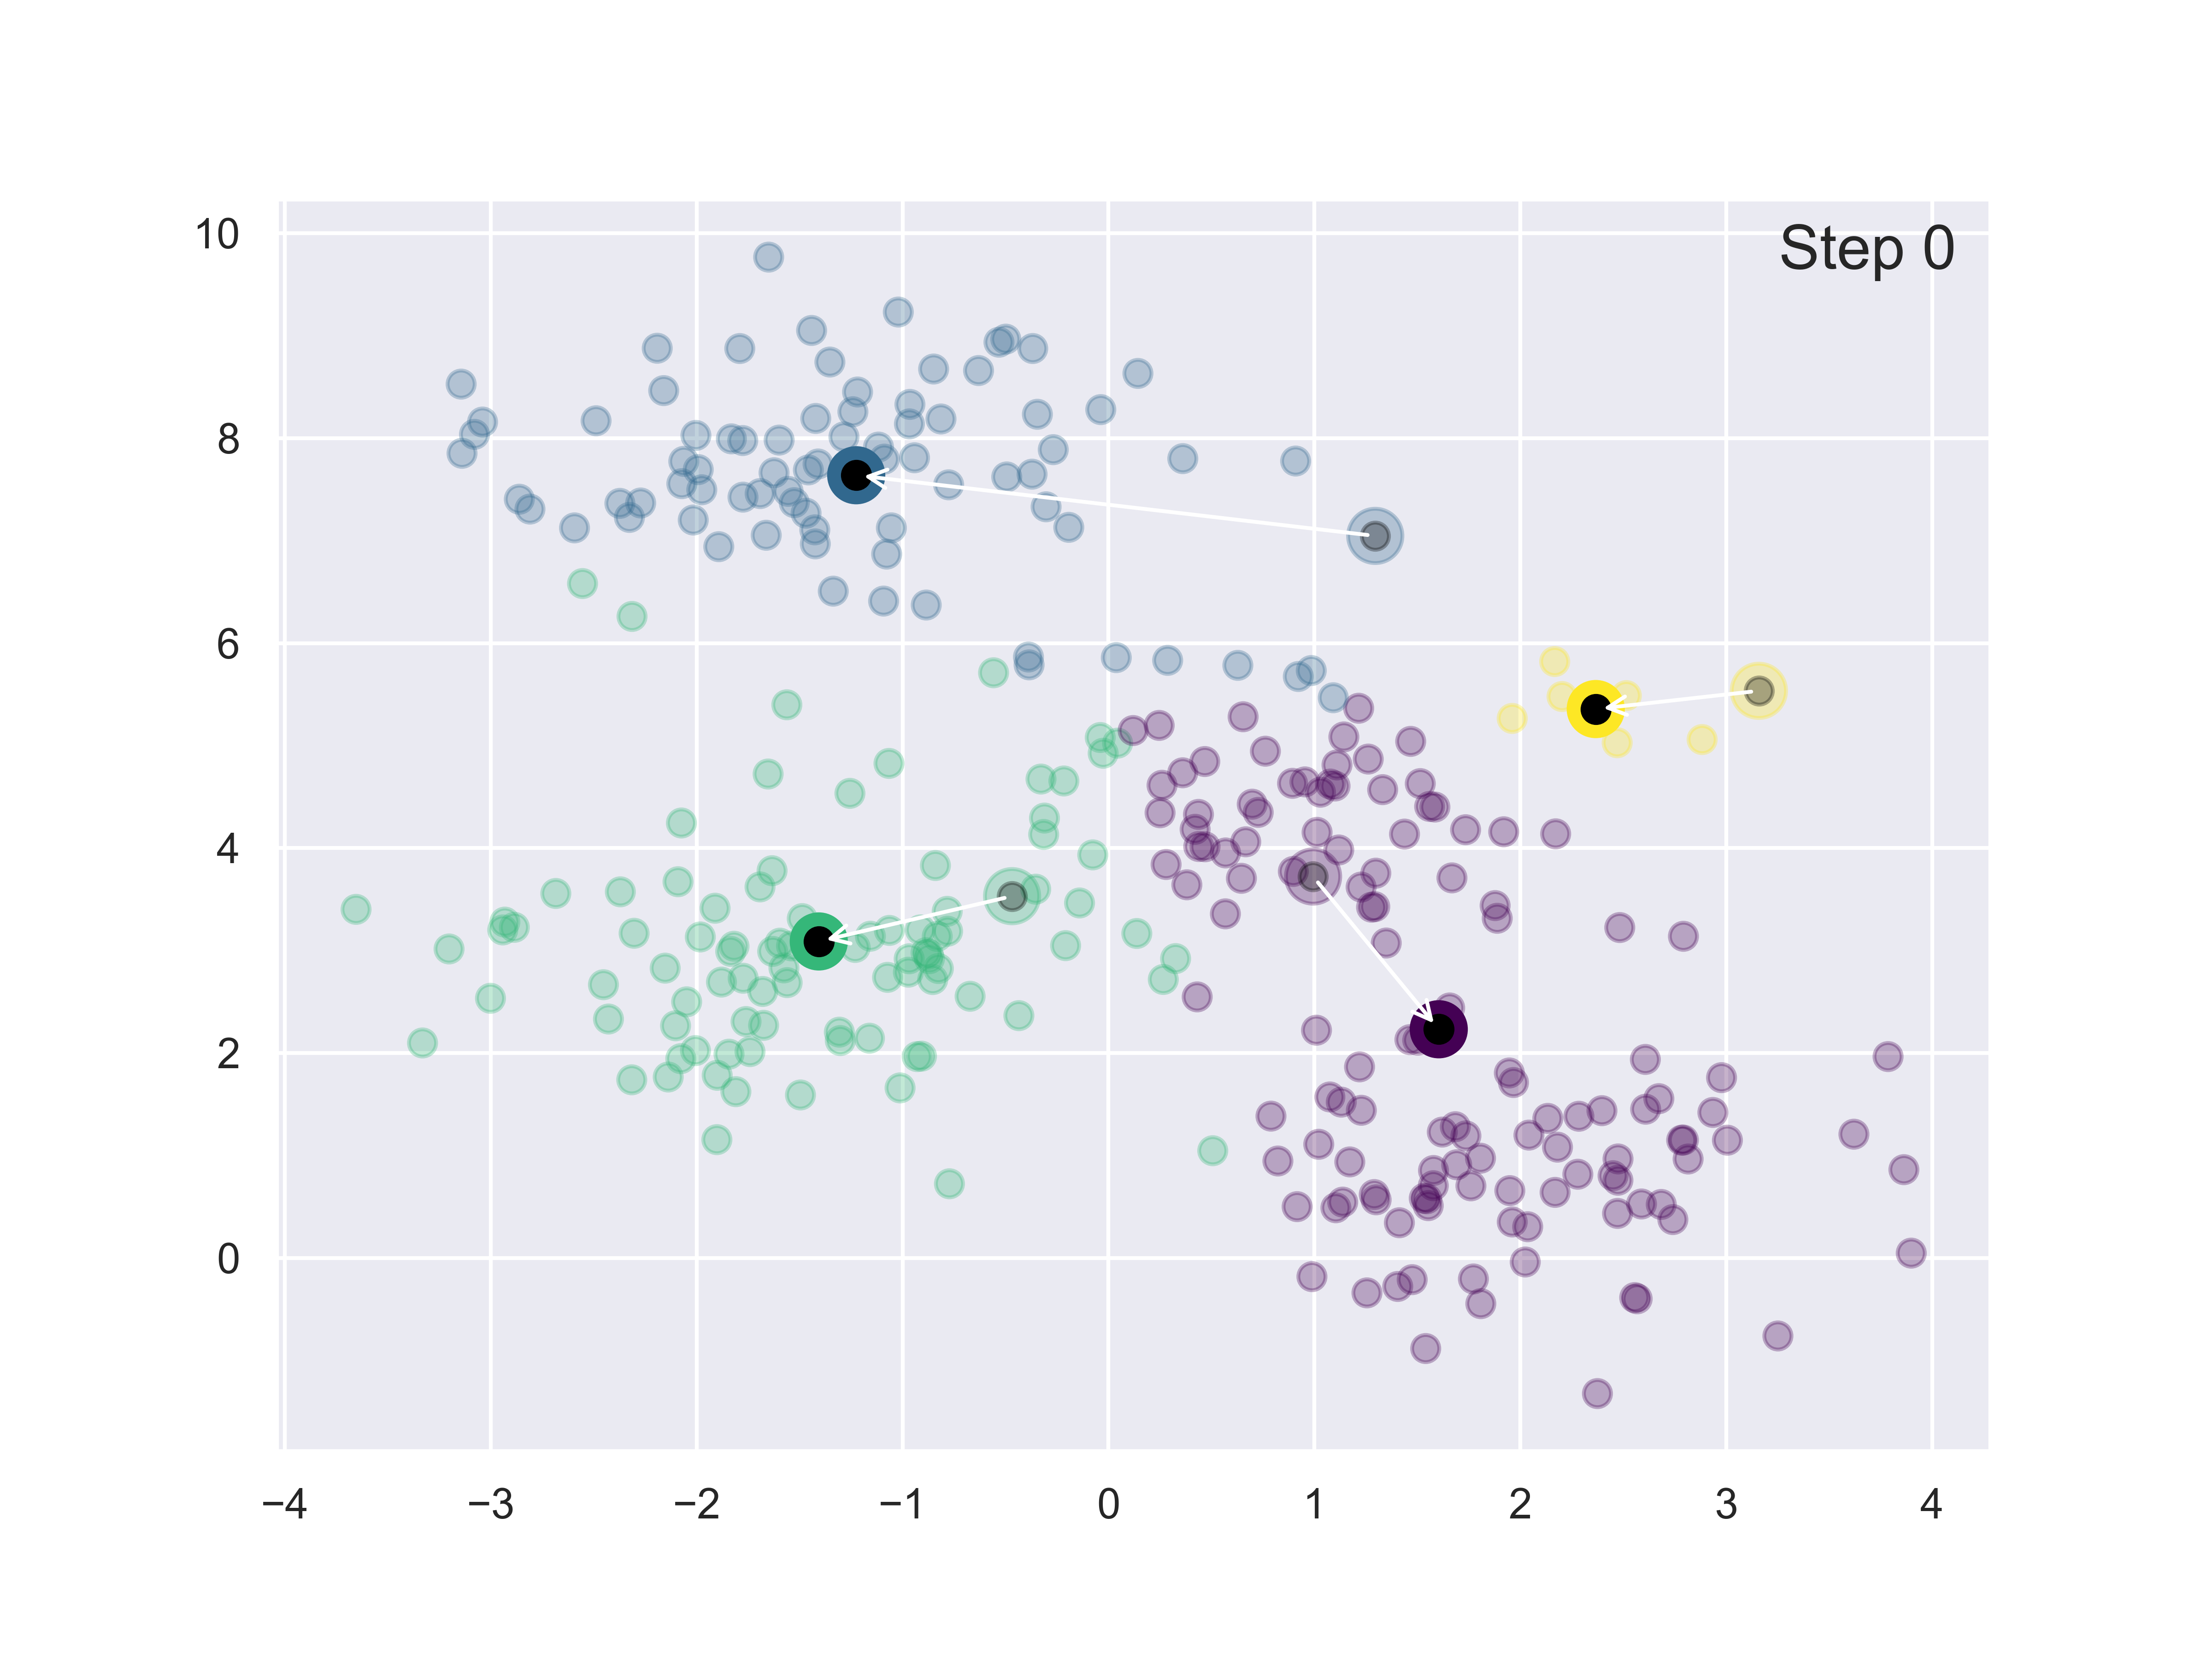
\includegraphics[width=0.7\textwidth]{PCAprocedure1}\source{}}
			\only<3>{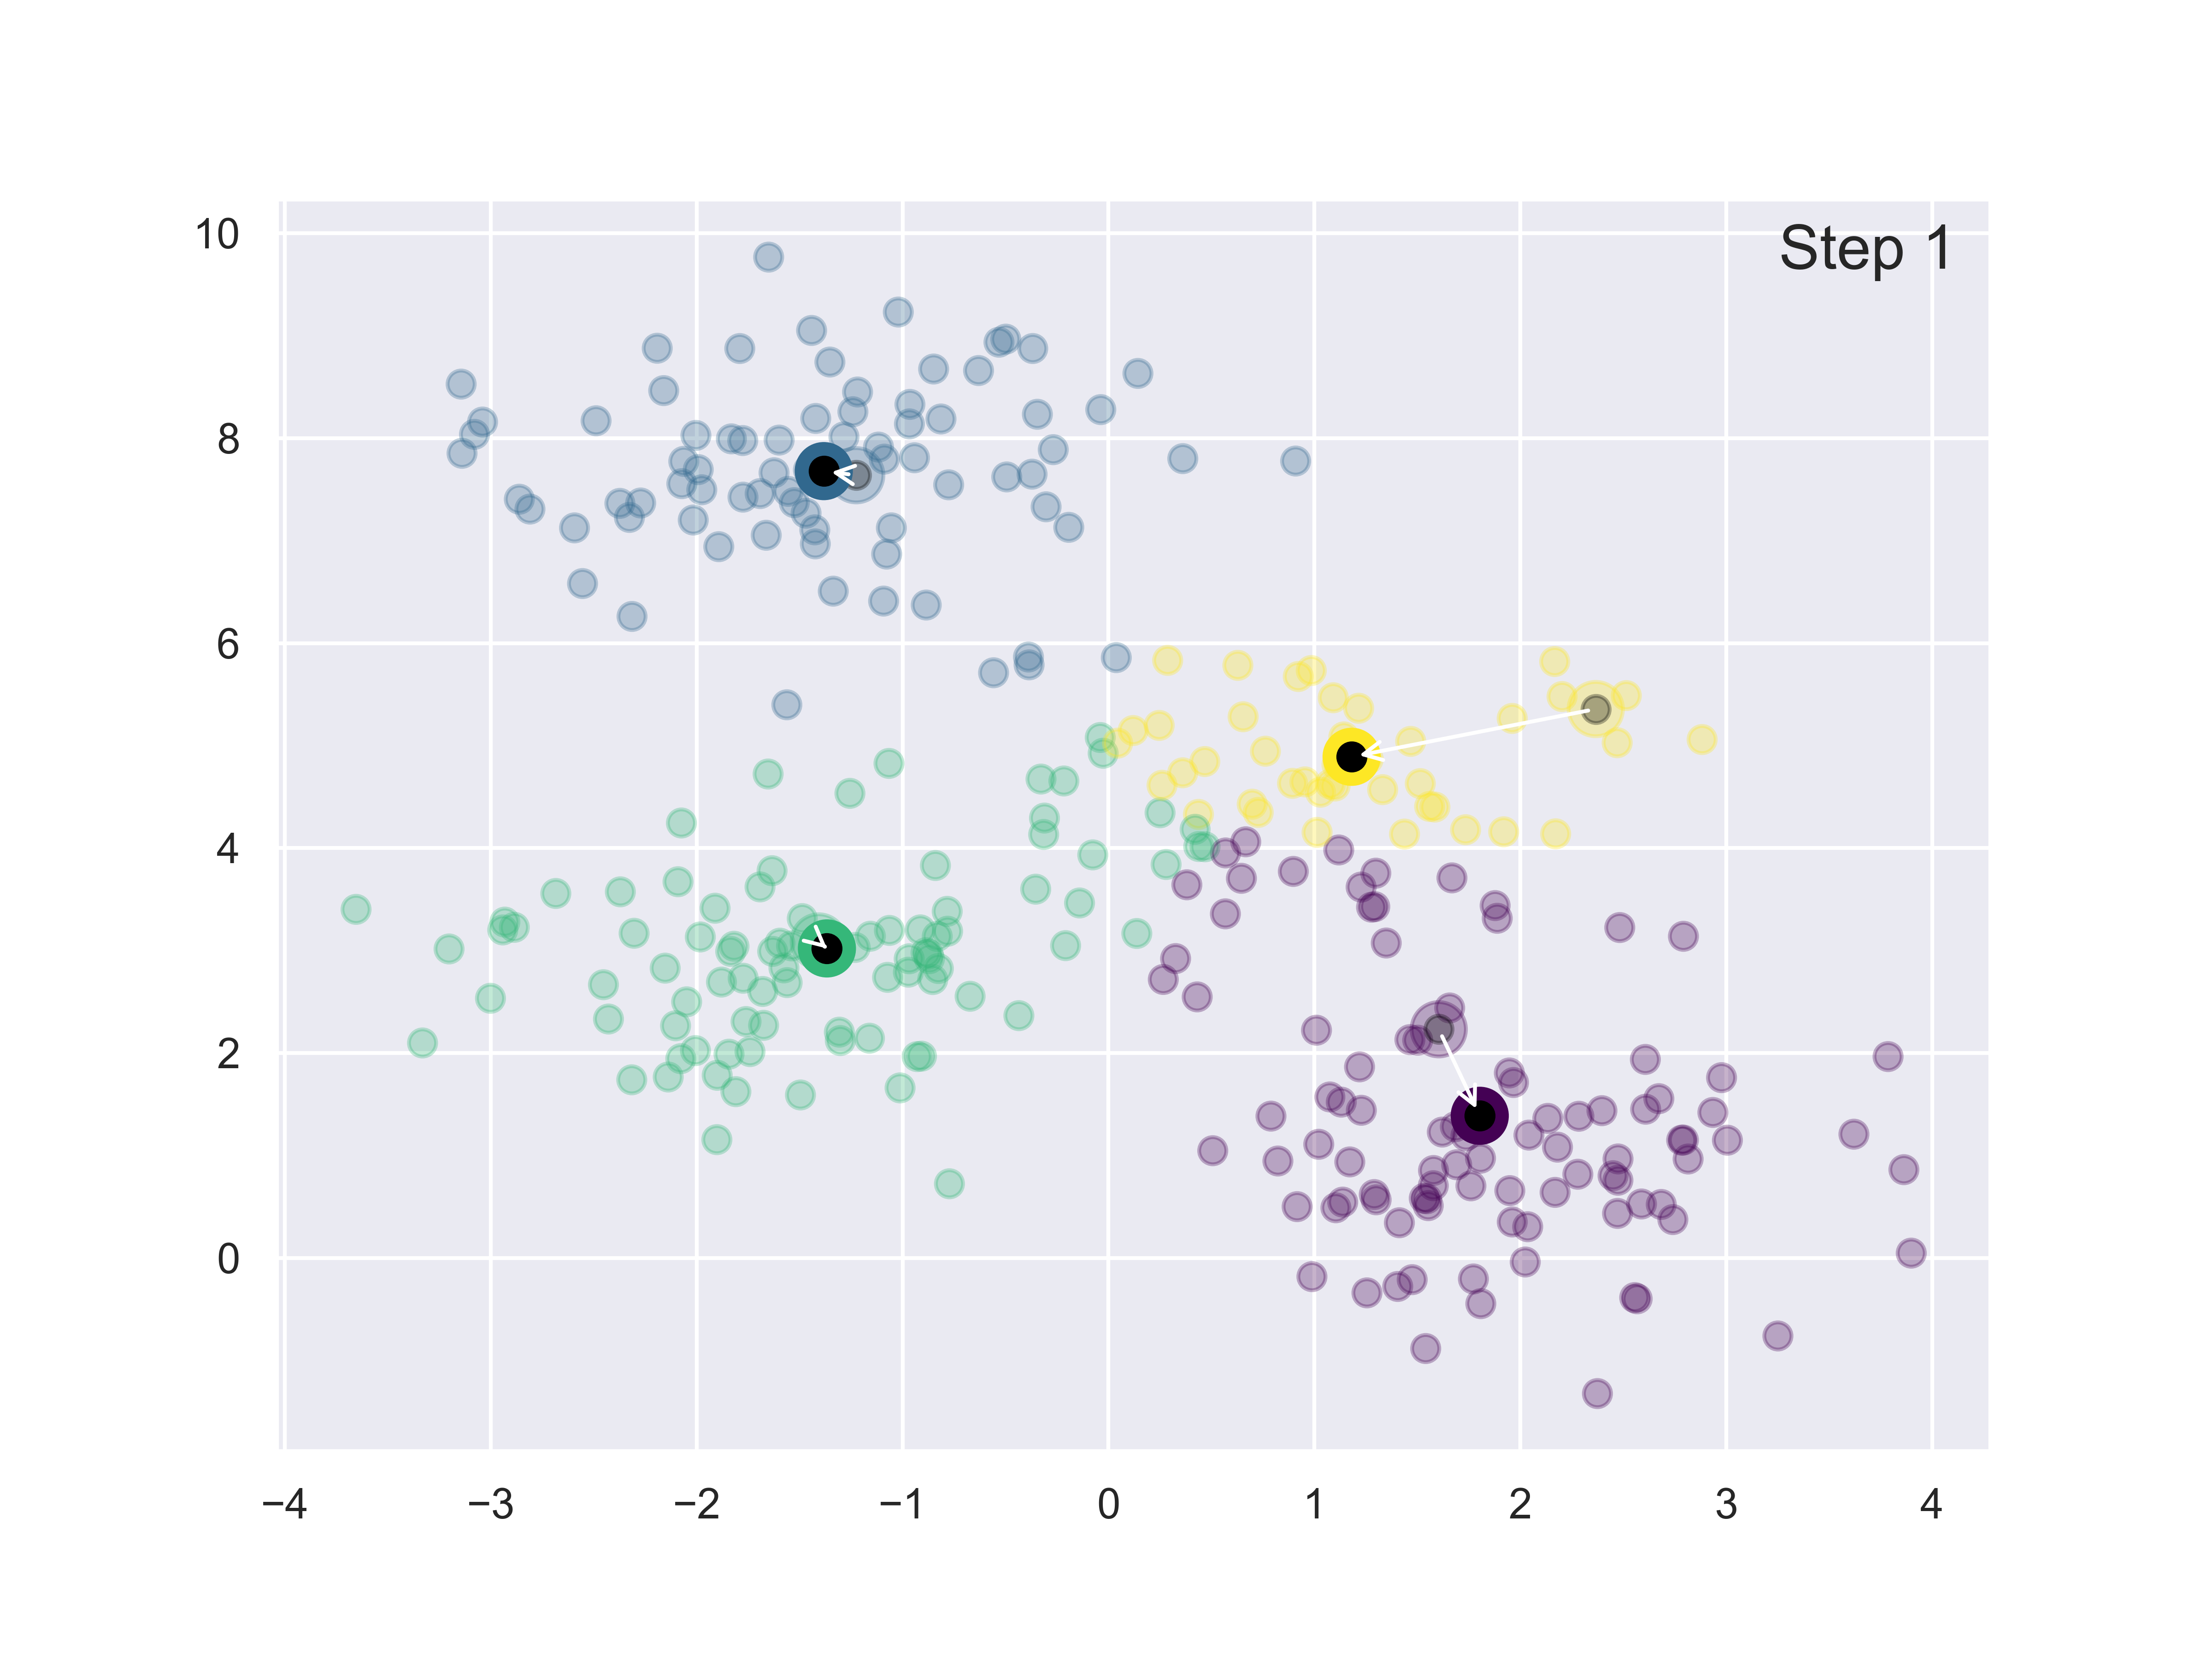
\includegraphics[width=0.7\textwidth]{PCAprocedure2}\source{}}
			\only<4>{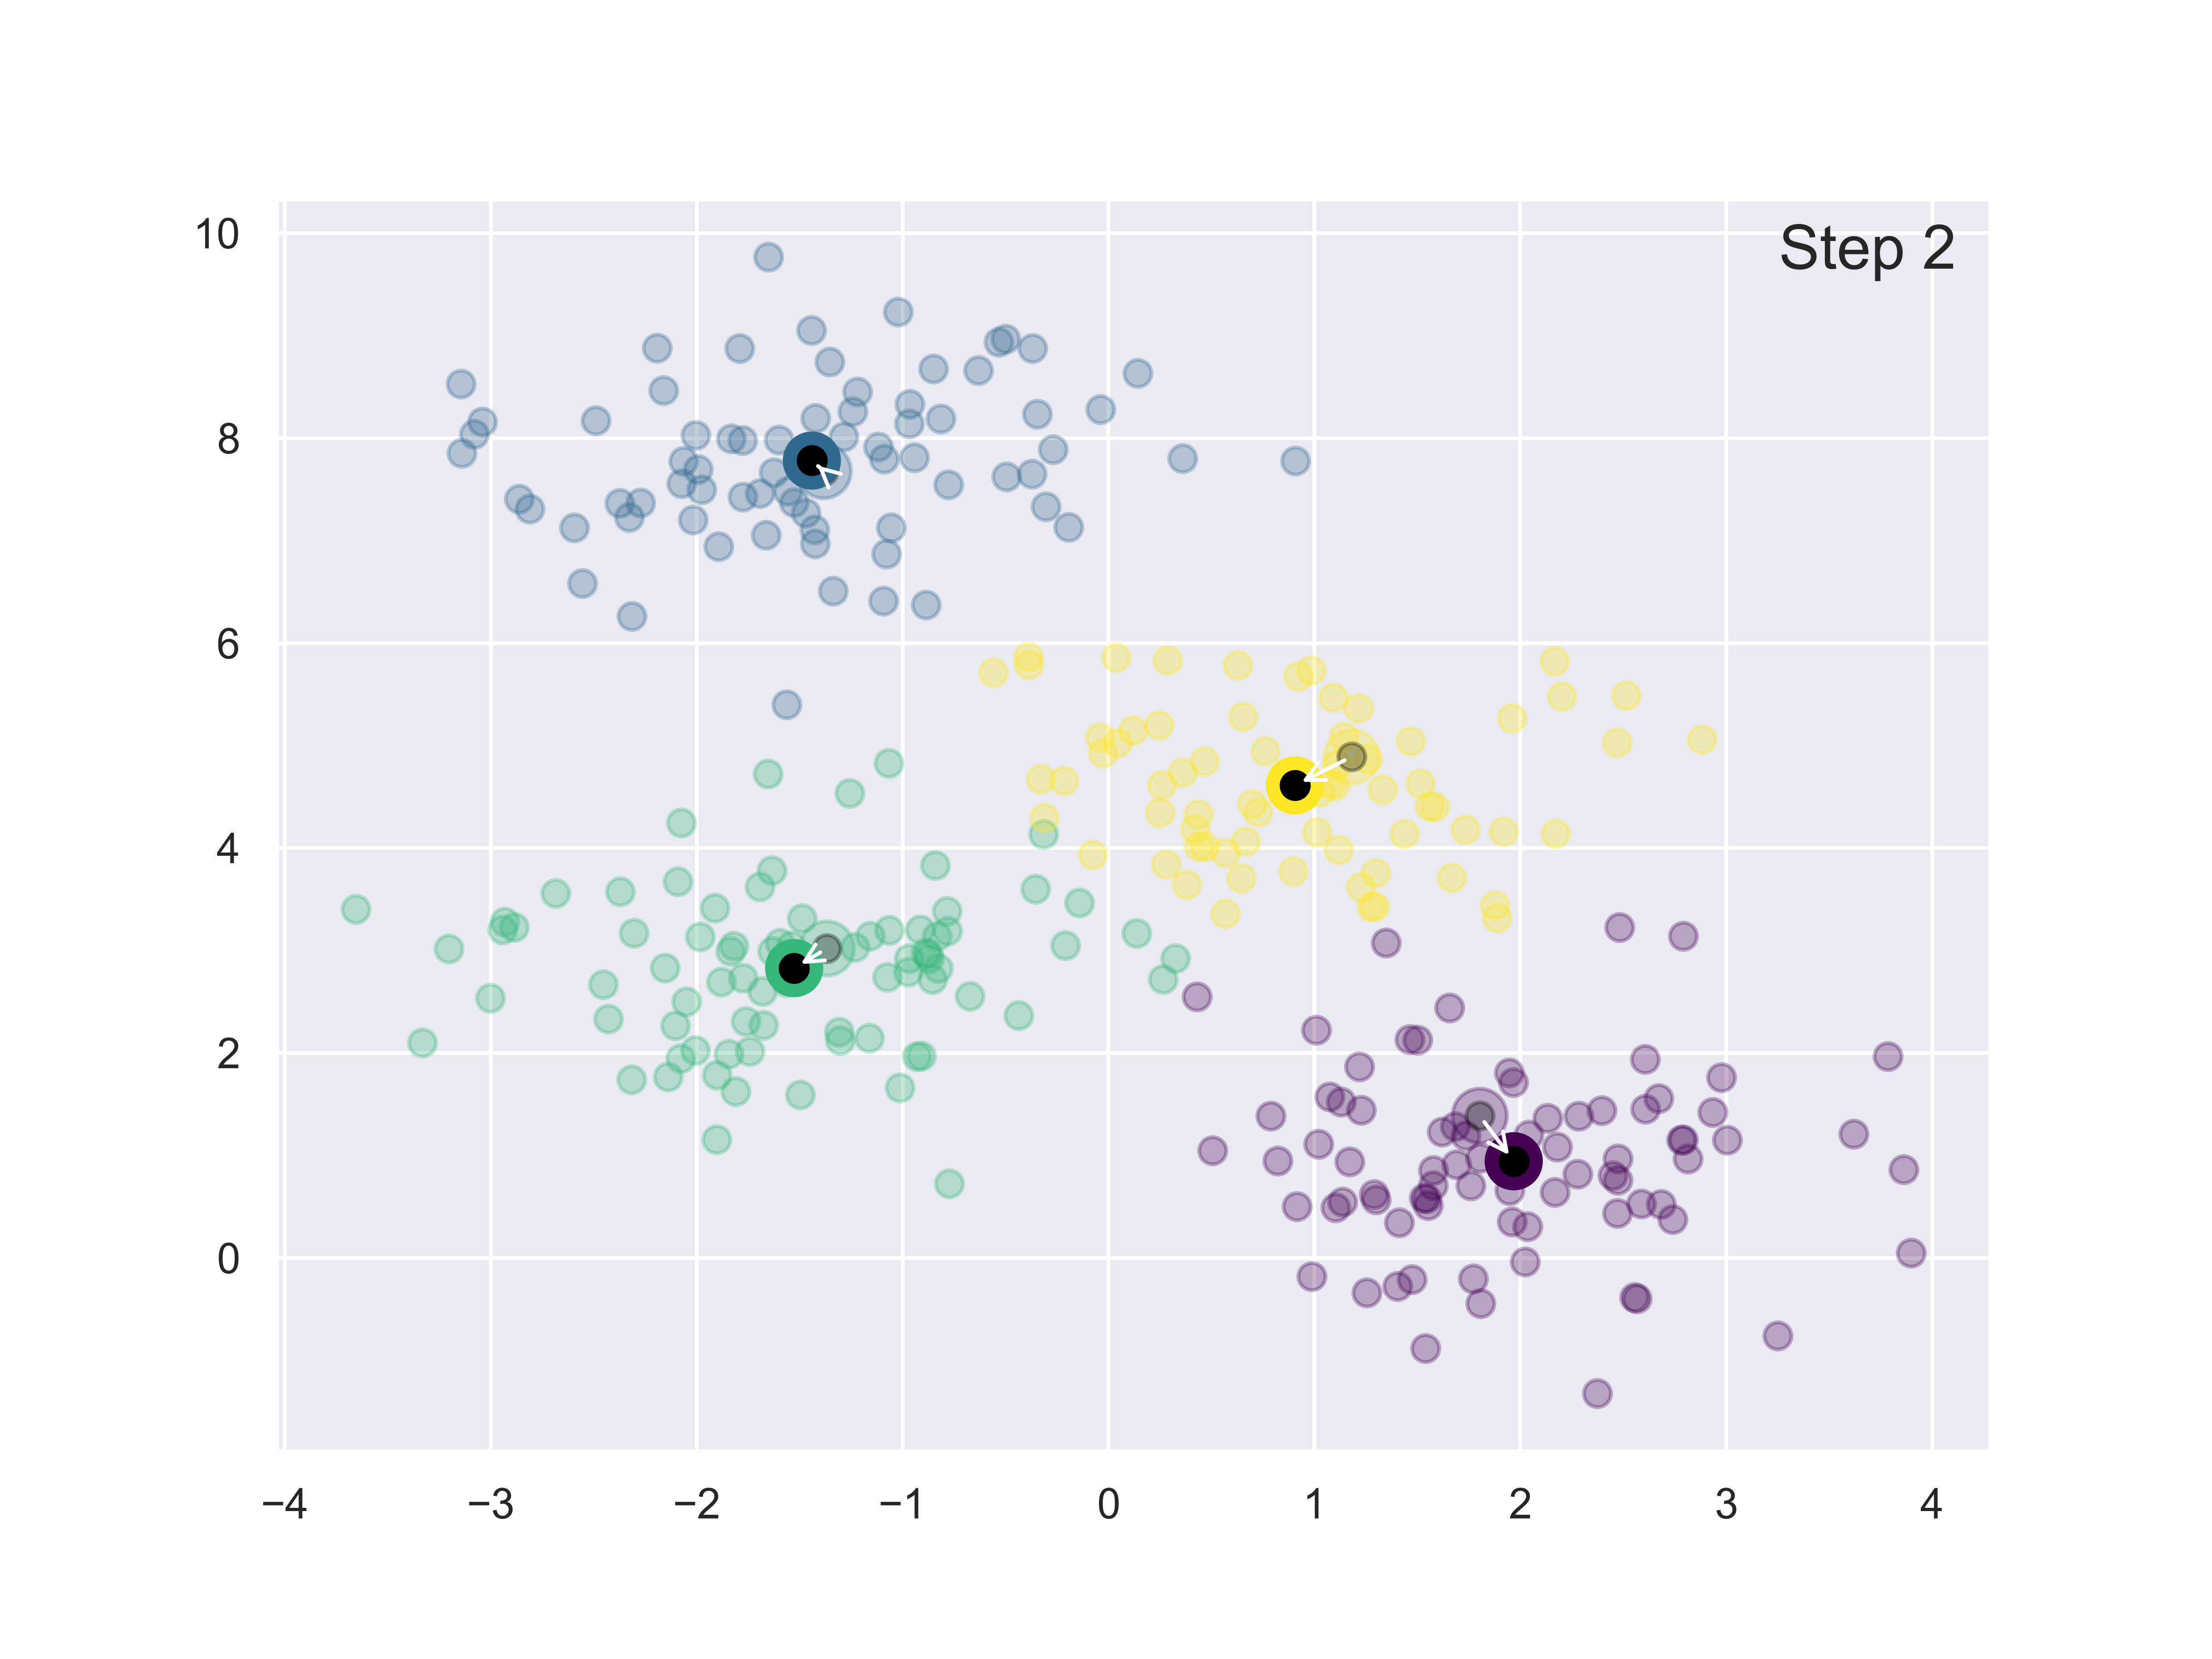
\includegraphics[width=0.7\textwidth]{PCAprocedure3}\source{}}
			\only<5>{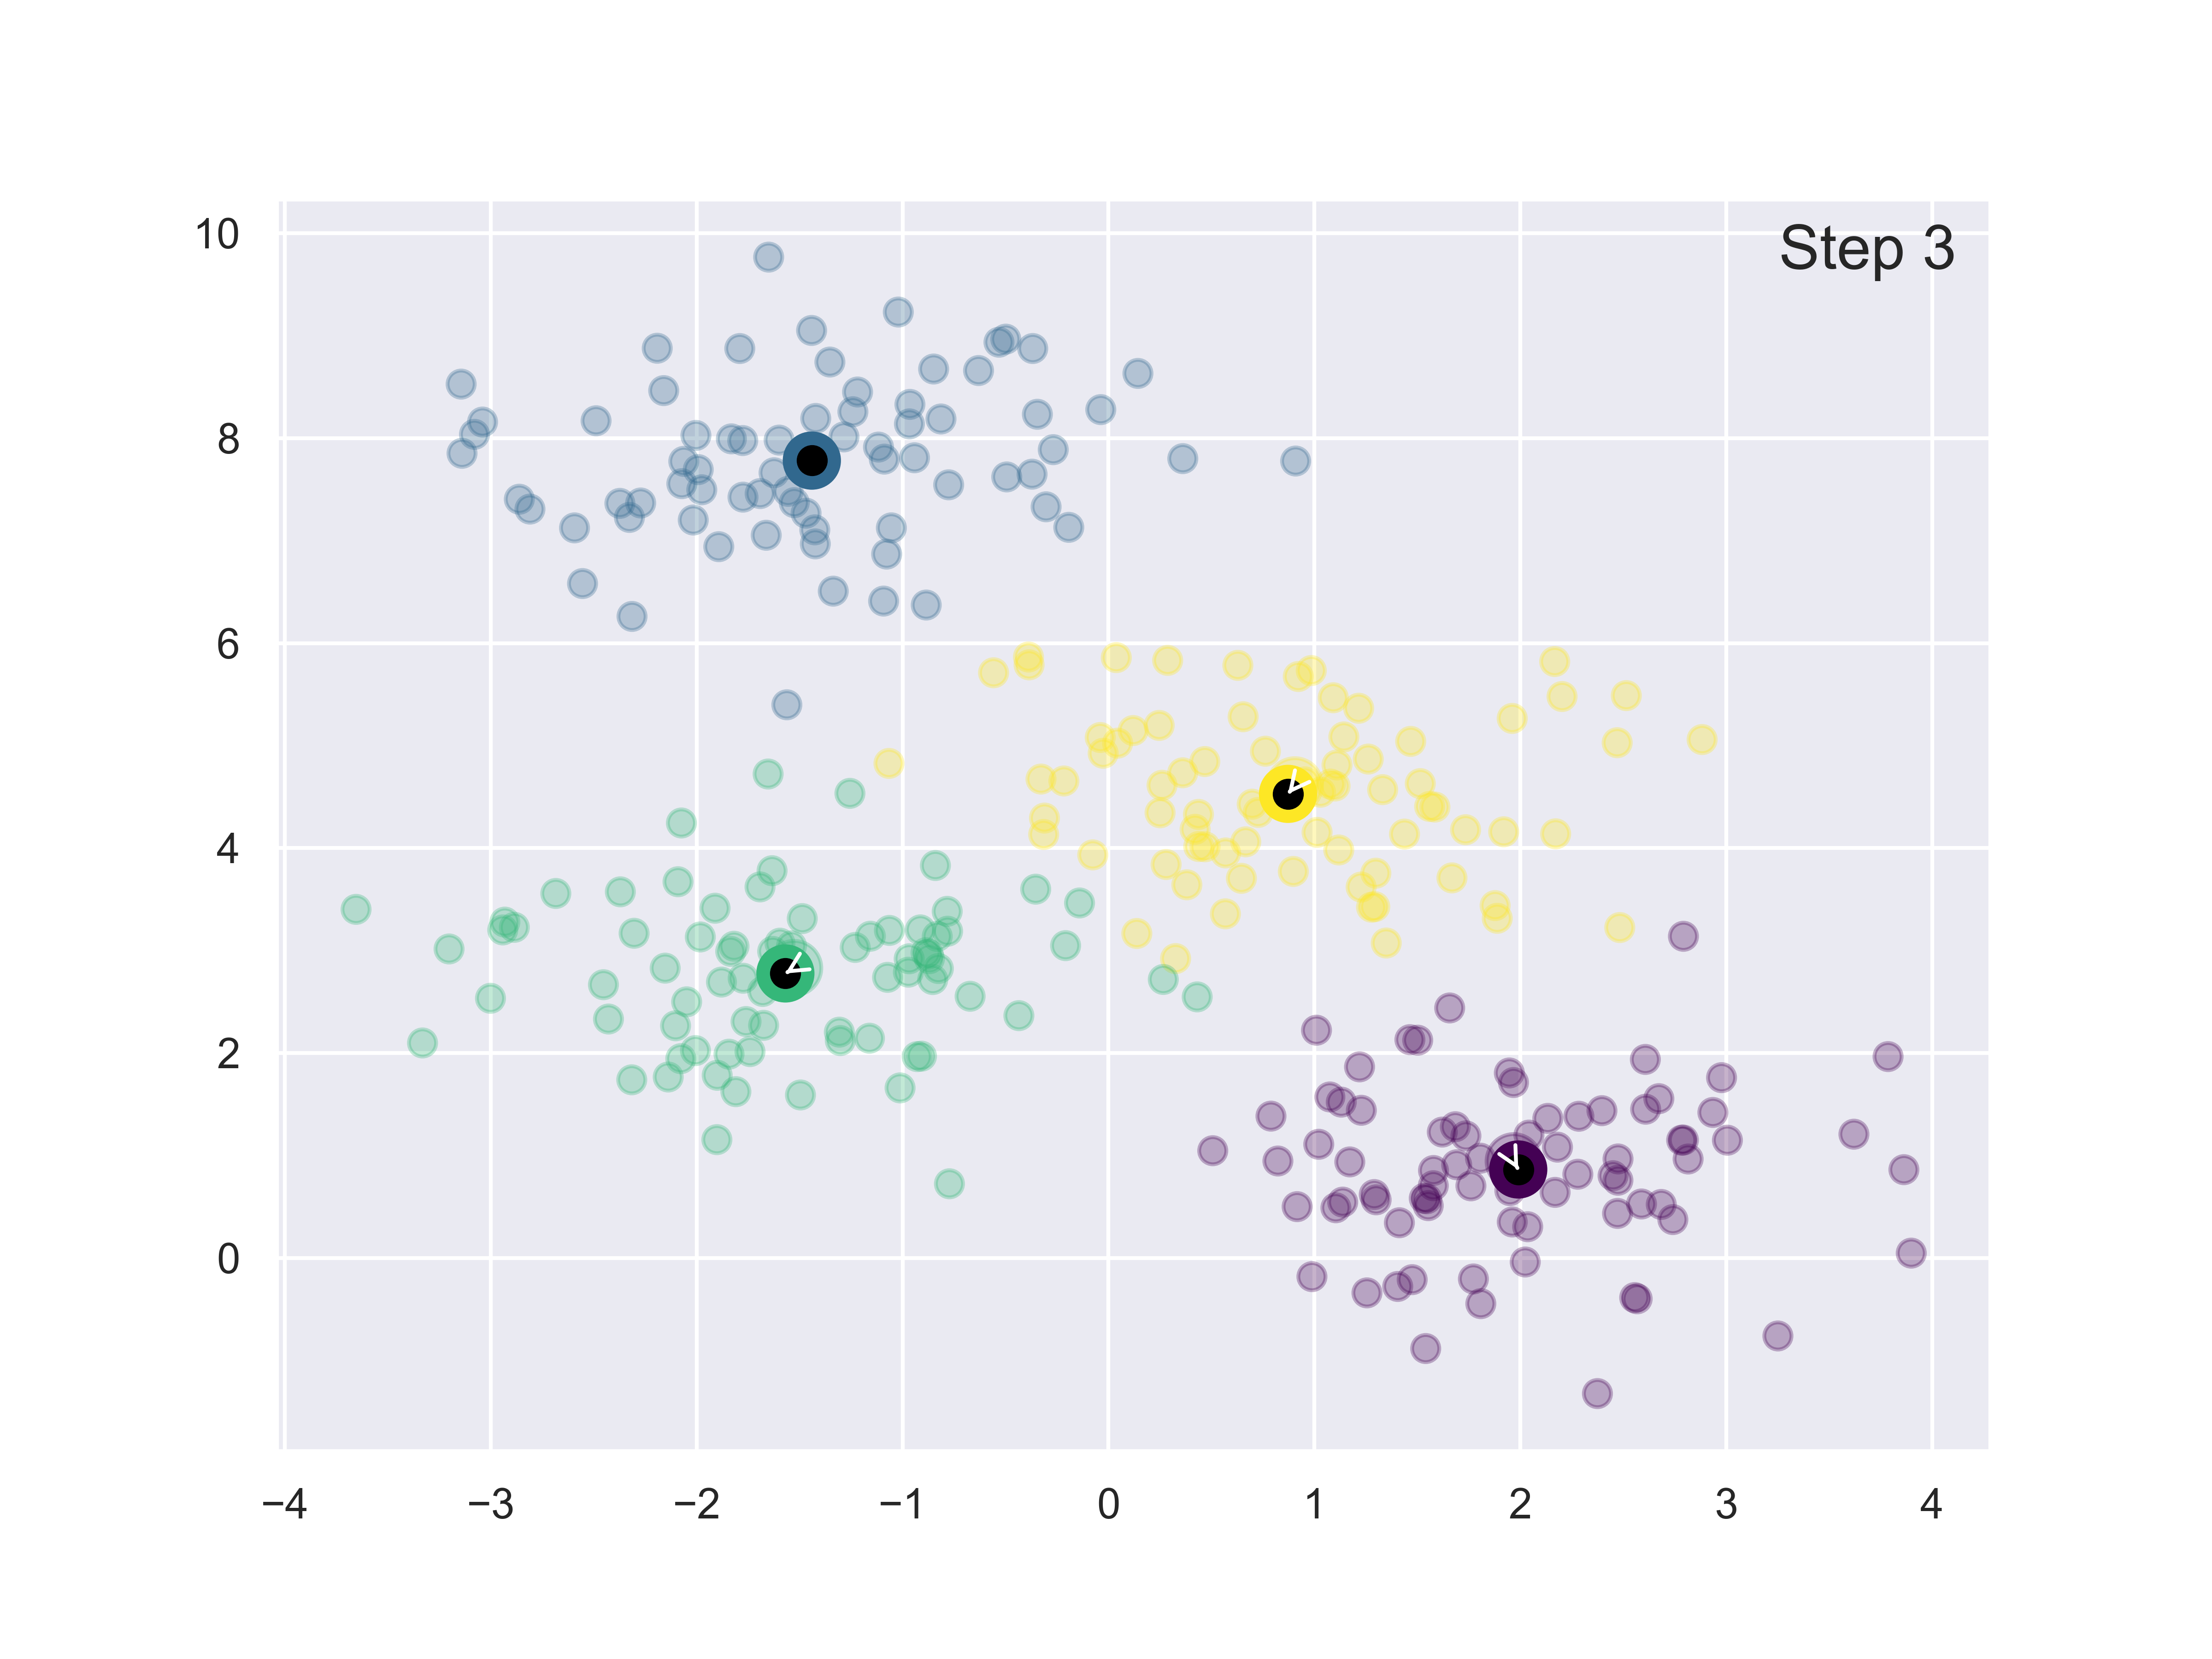
\includegraphics[width=0.7\textwidth]{PCAprocedure4}\source{}}
			\only<6>{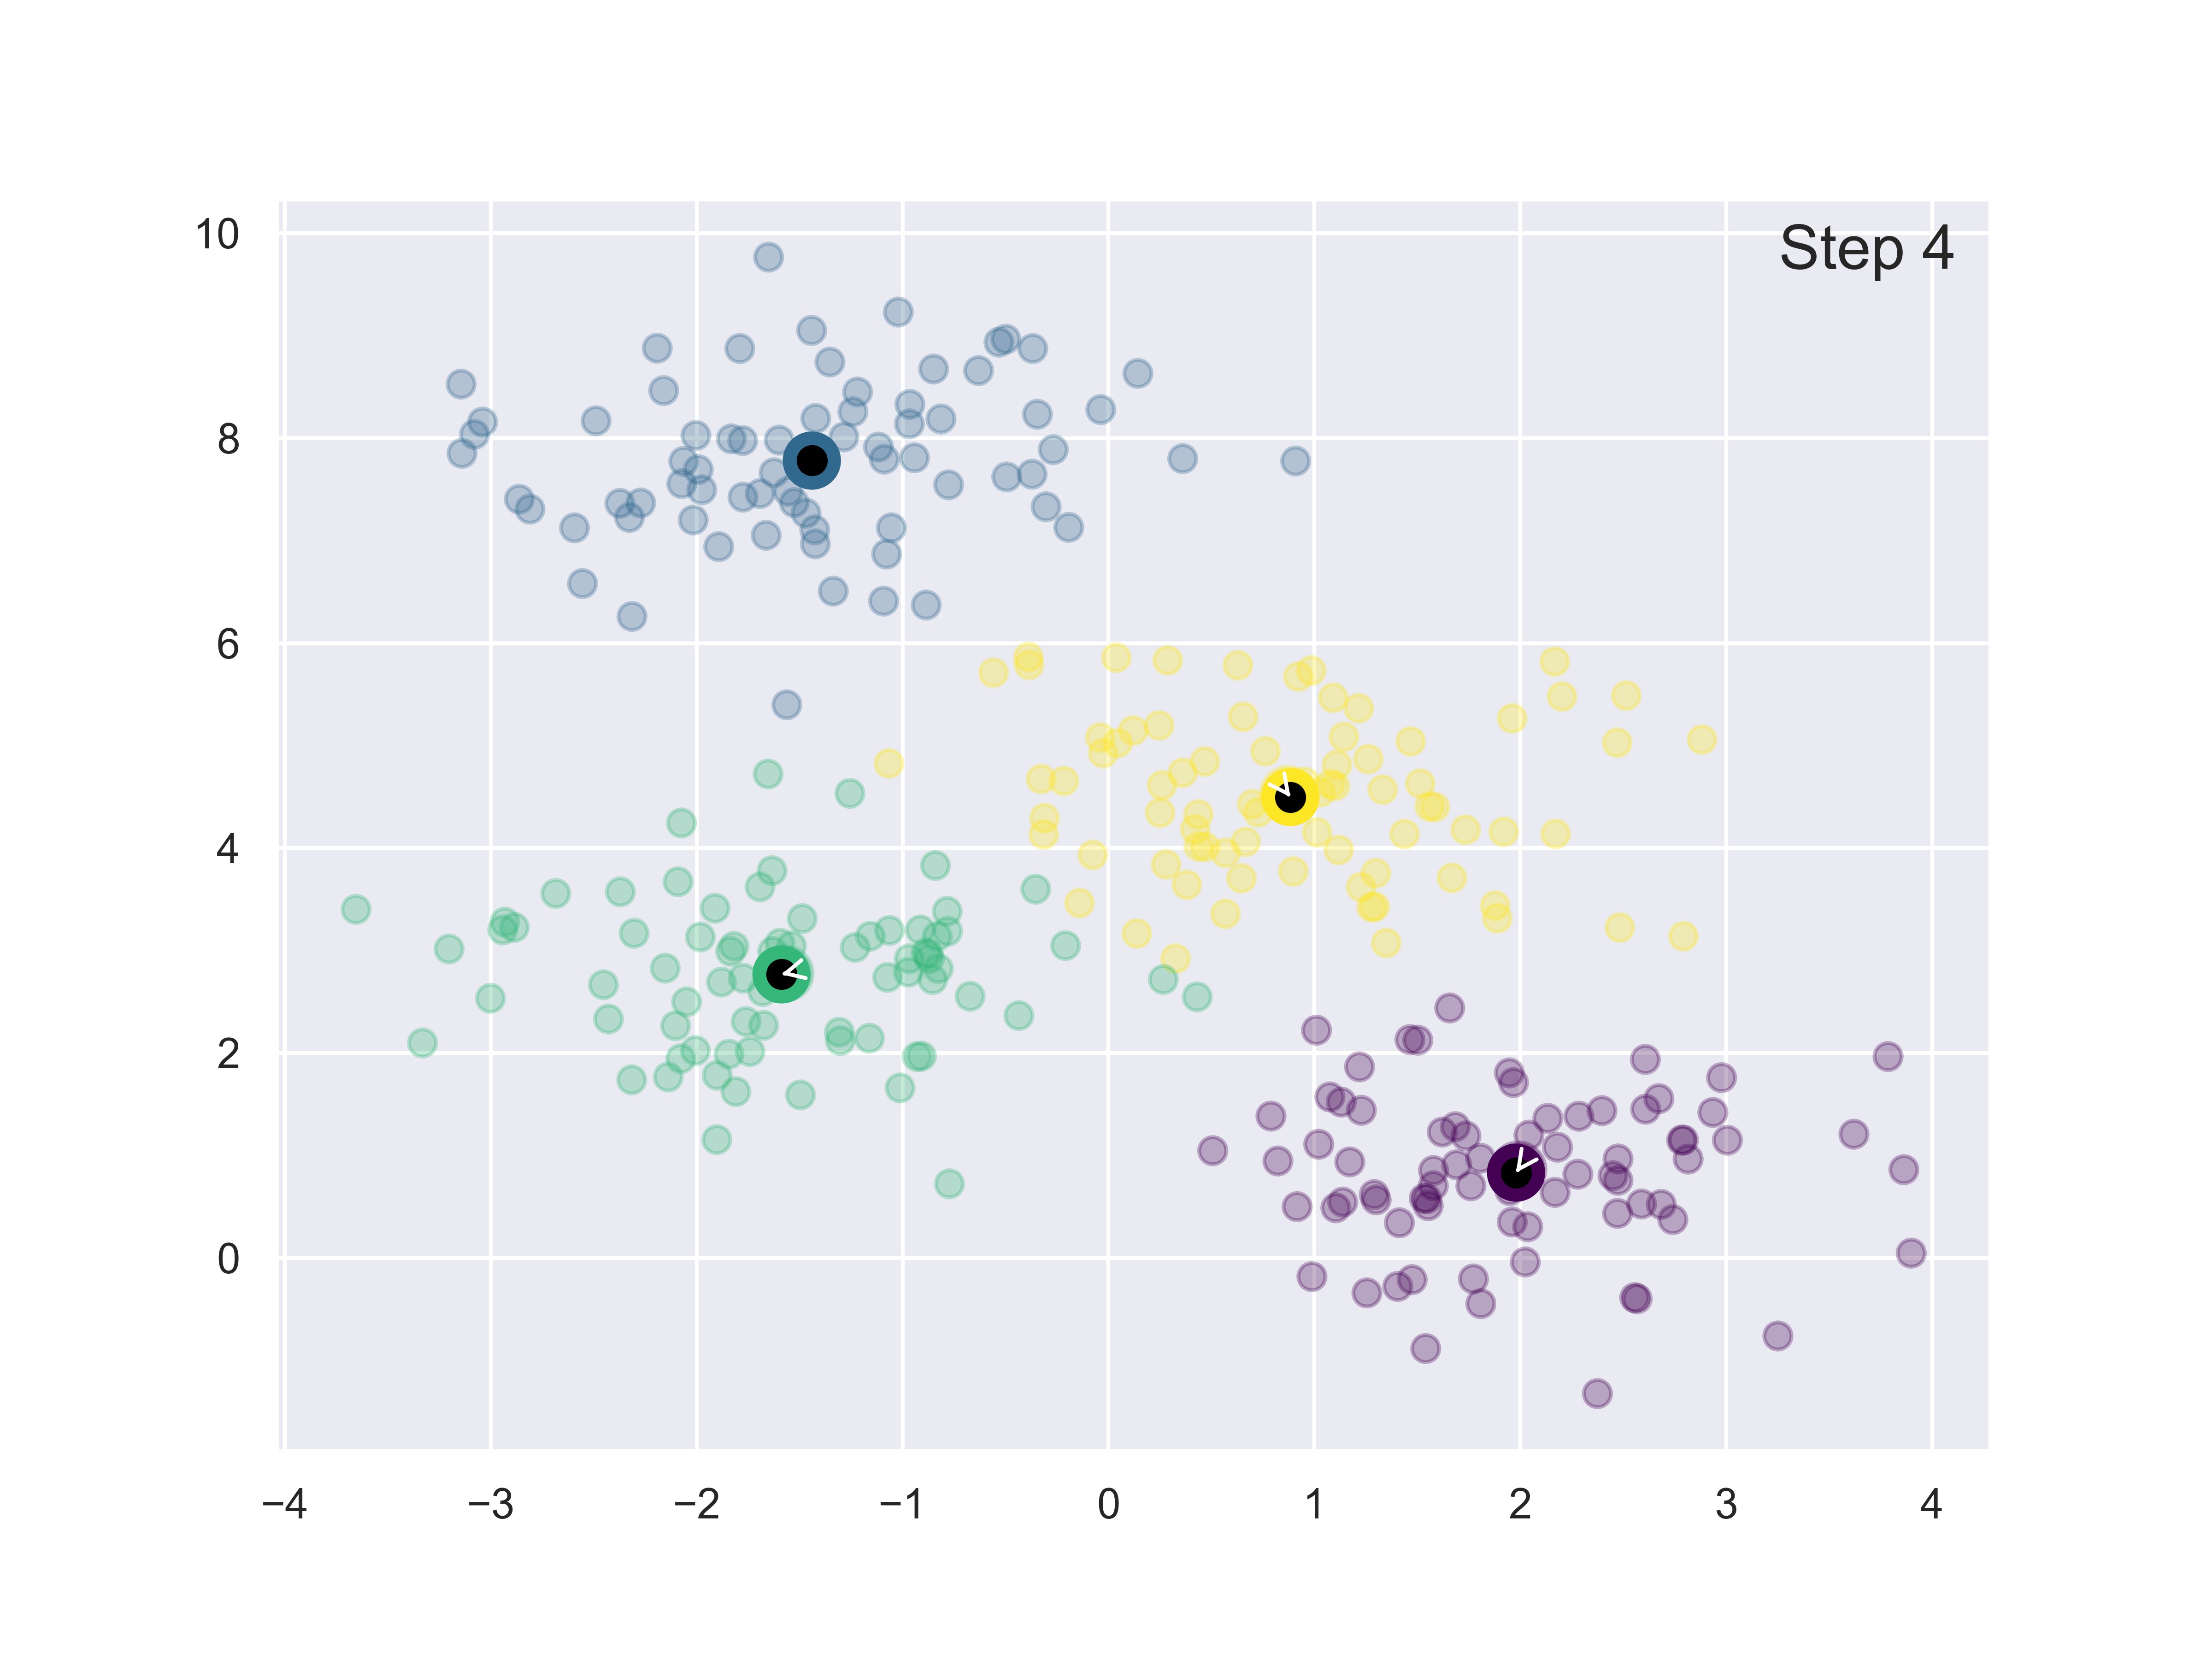
\includegraphics[width=0.7\textwidth]{PCAprocedure5}\source{}}
			%\only<7>{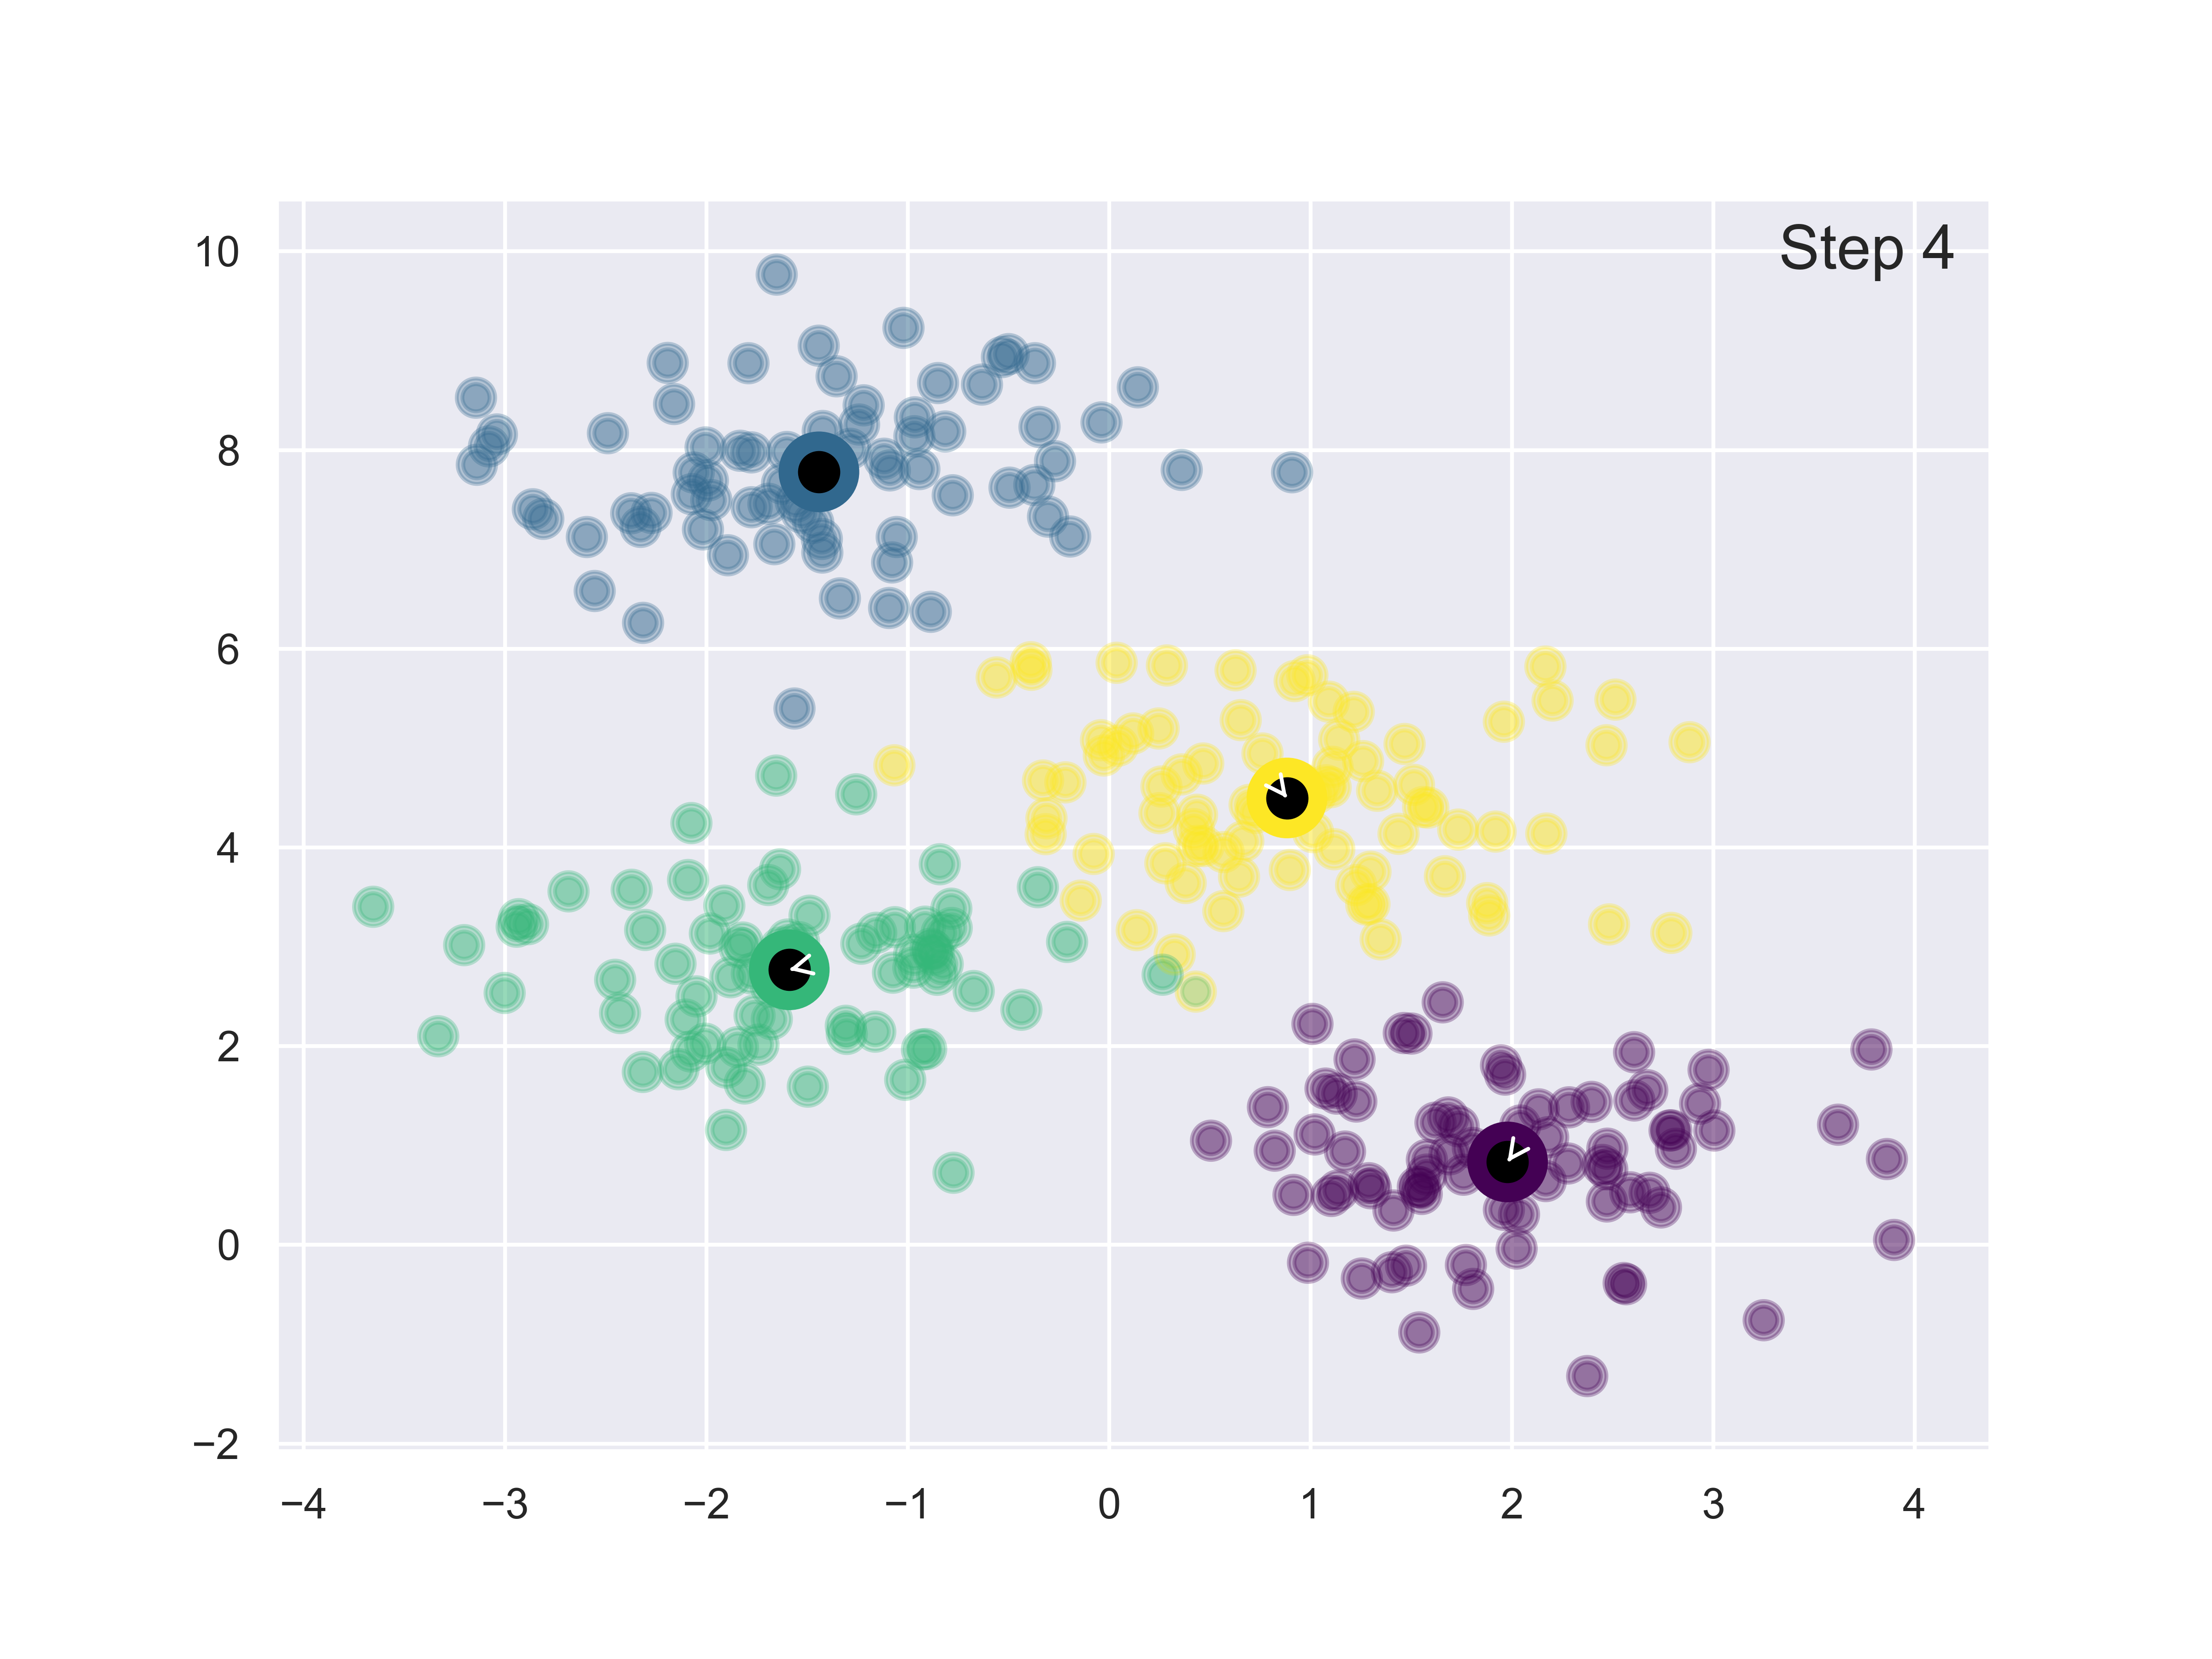
\includegraphics[width=0.7\textwidth]{PCAprocedure6}\source{}}

        		\end{center}}
		
\frame{\frametitle{K-means inappropriate cluster number}
         	\begin{center}
            		\only<1>{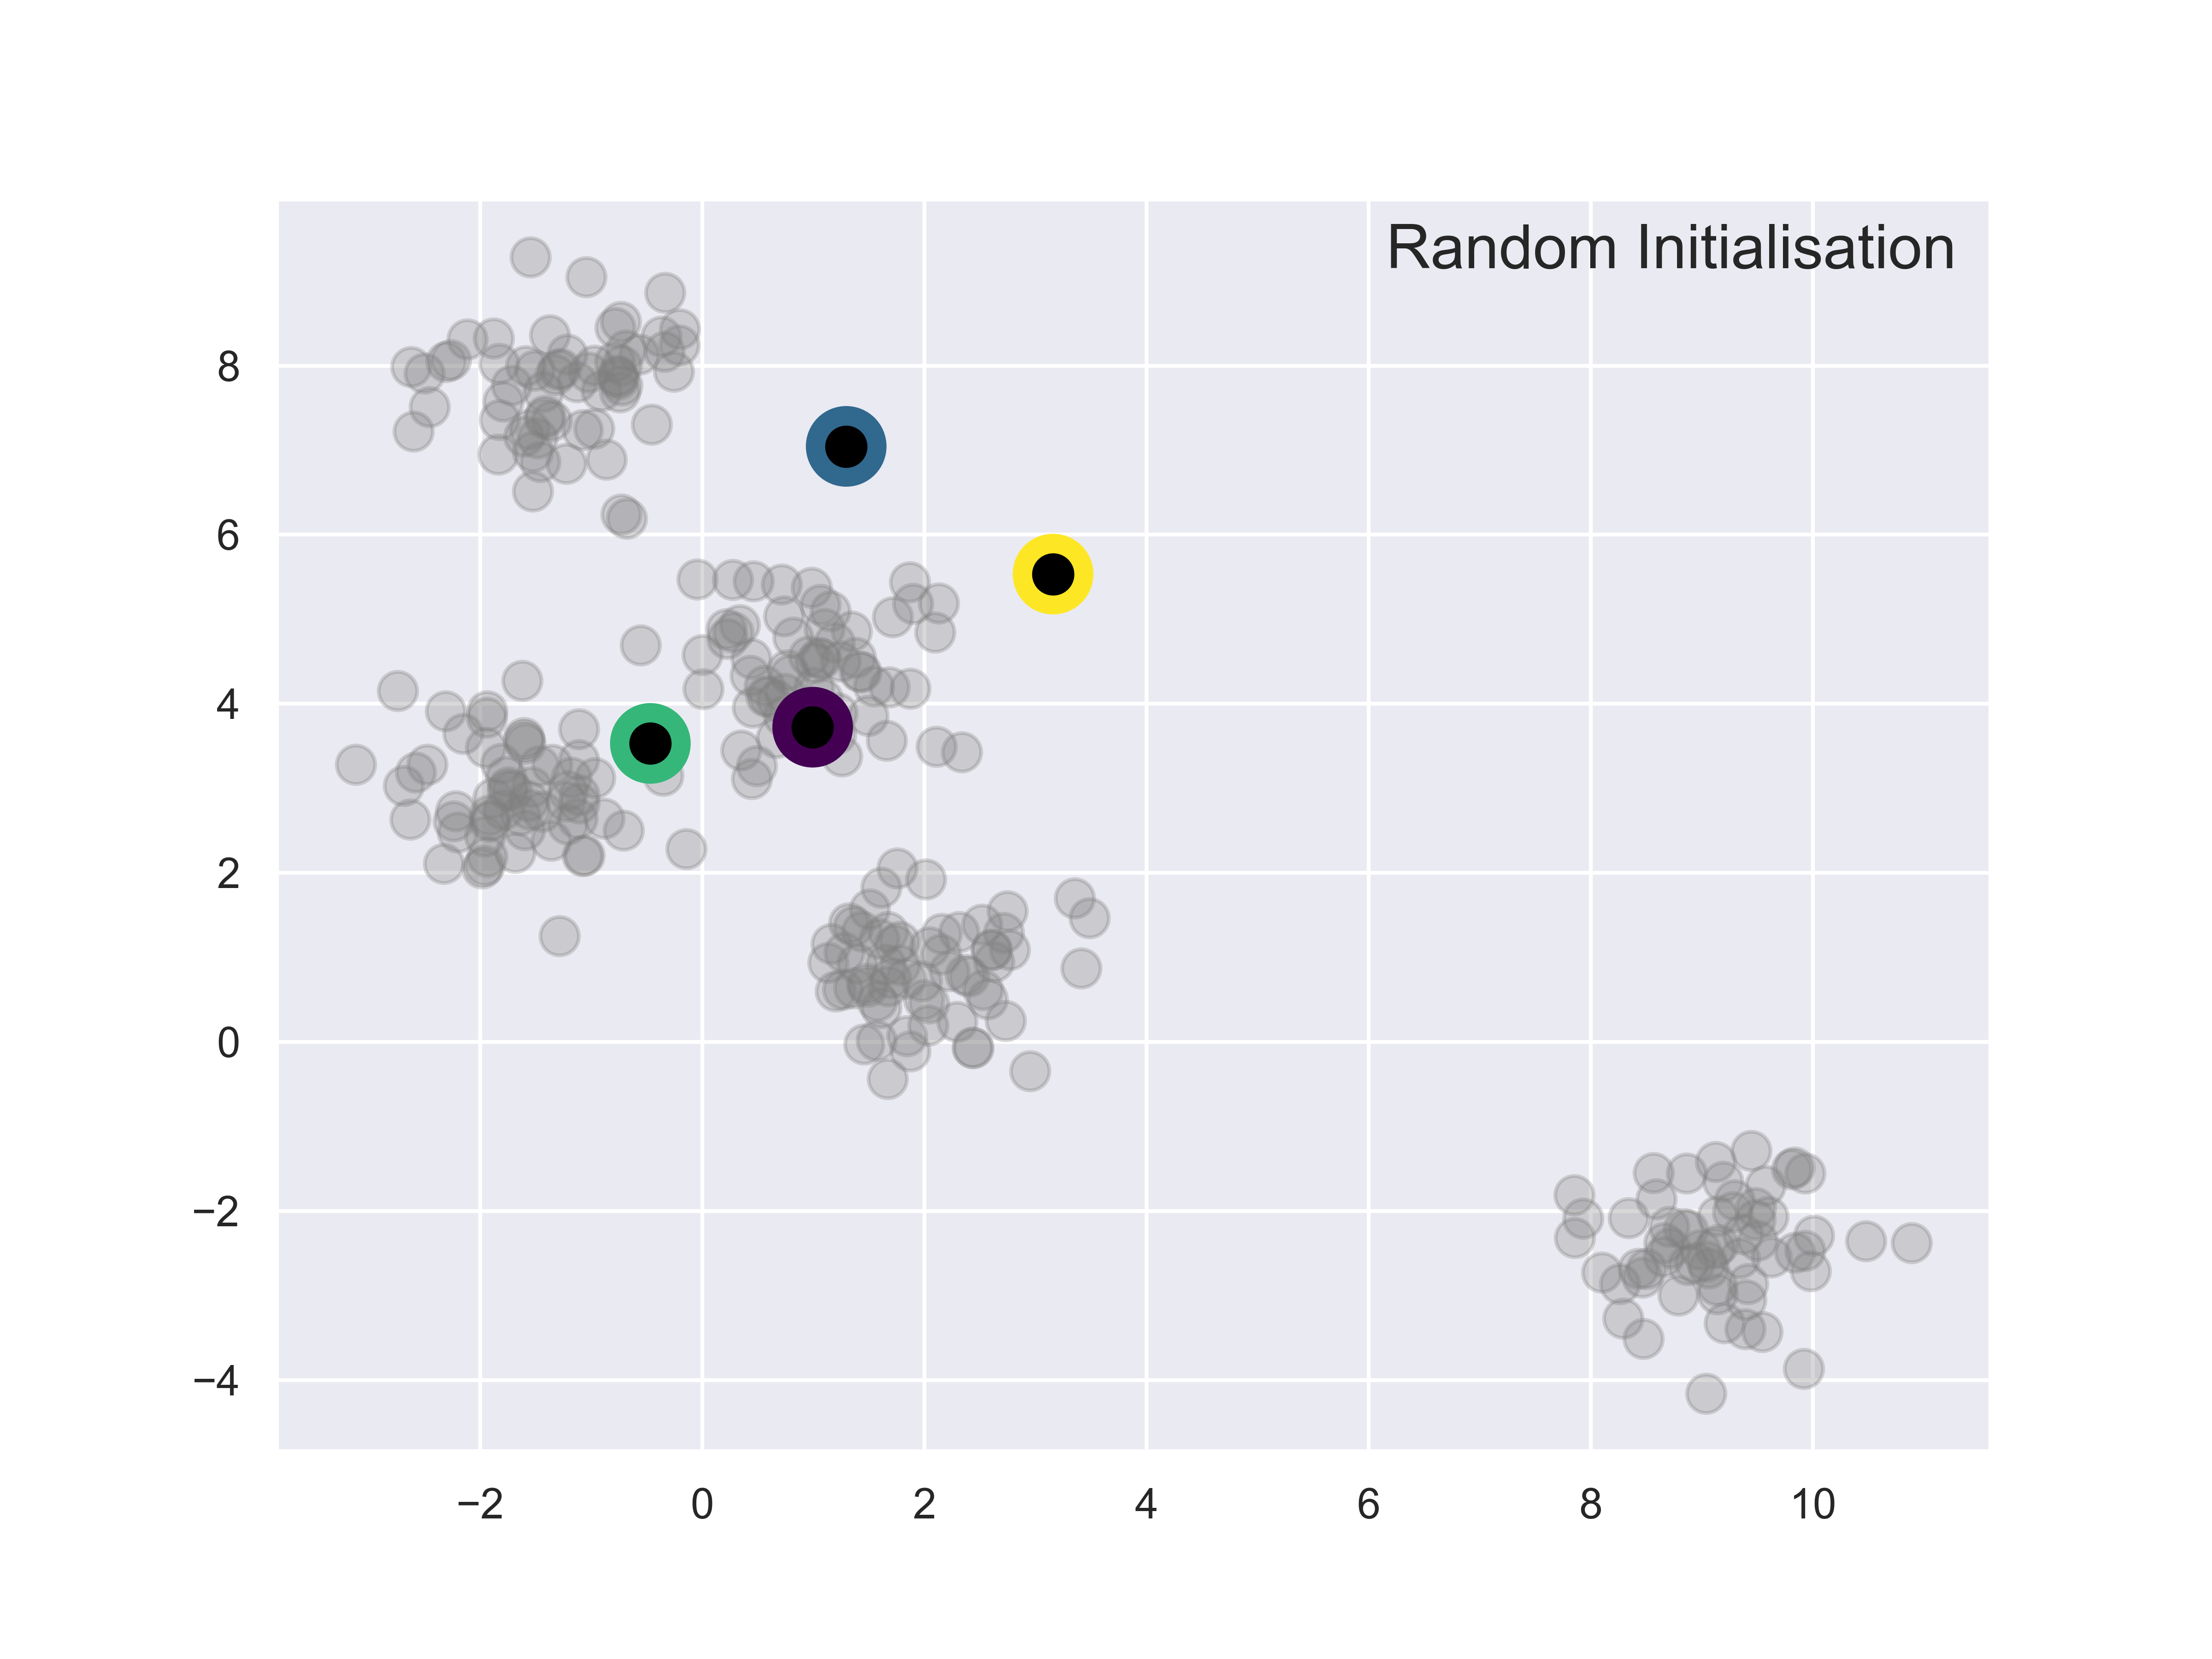
\includegraphics[width=0.7\textwidth]{PCAprocedureFewCluster0}\source{}}
			\only<2>{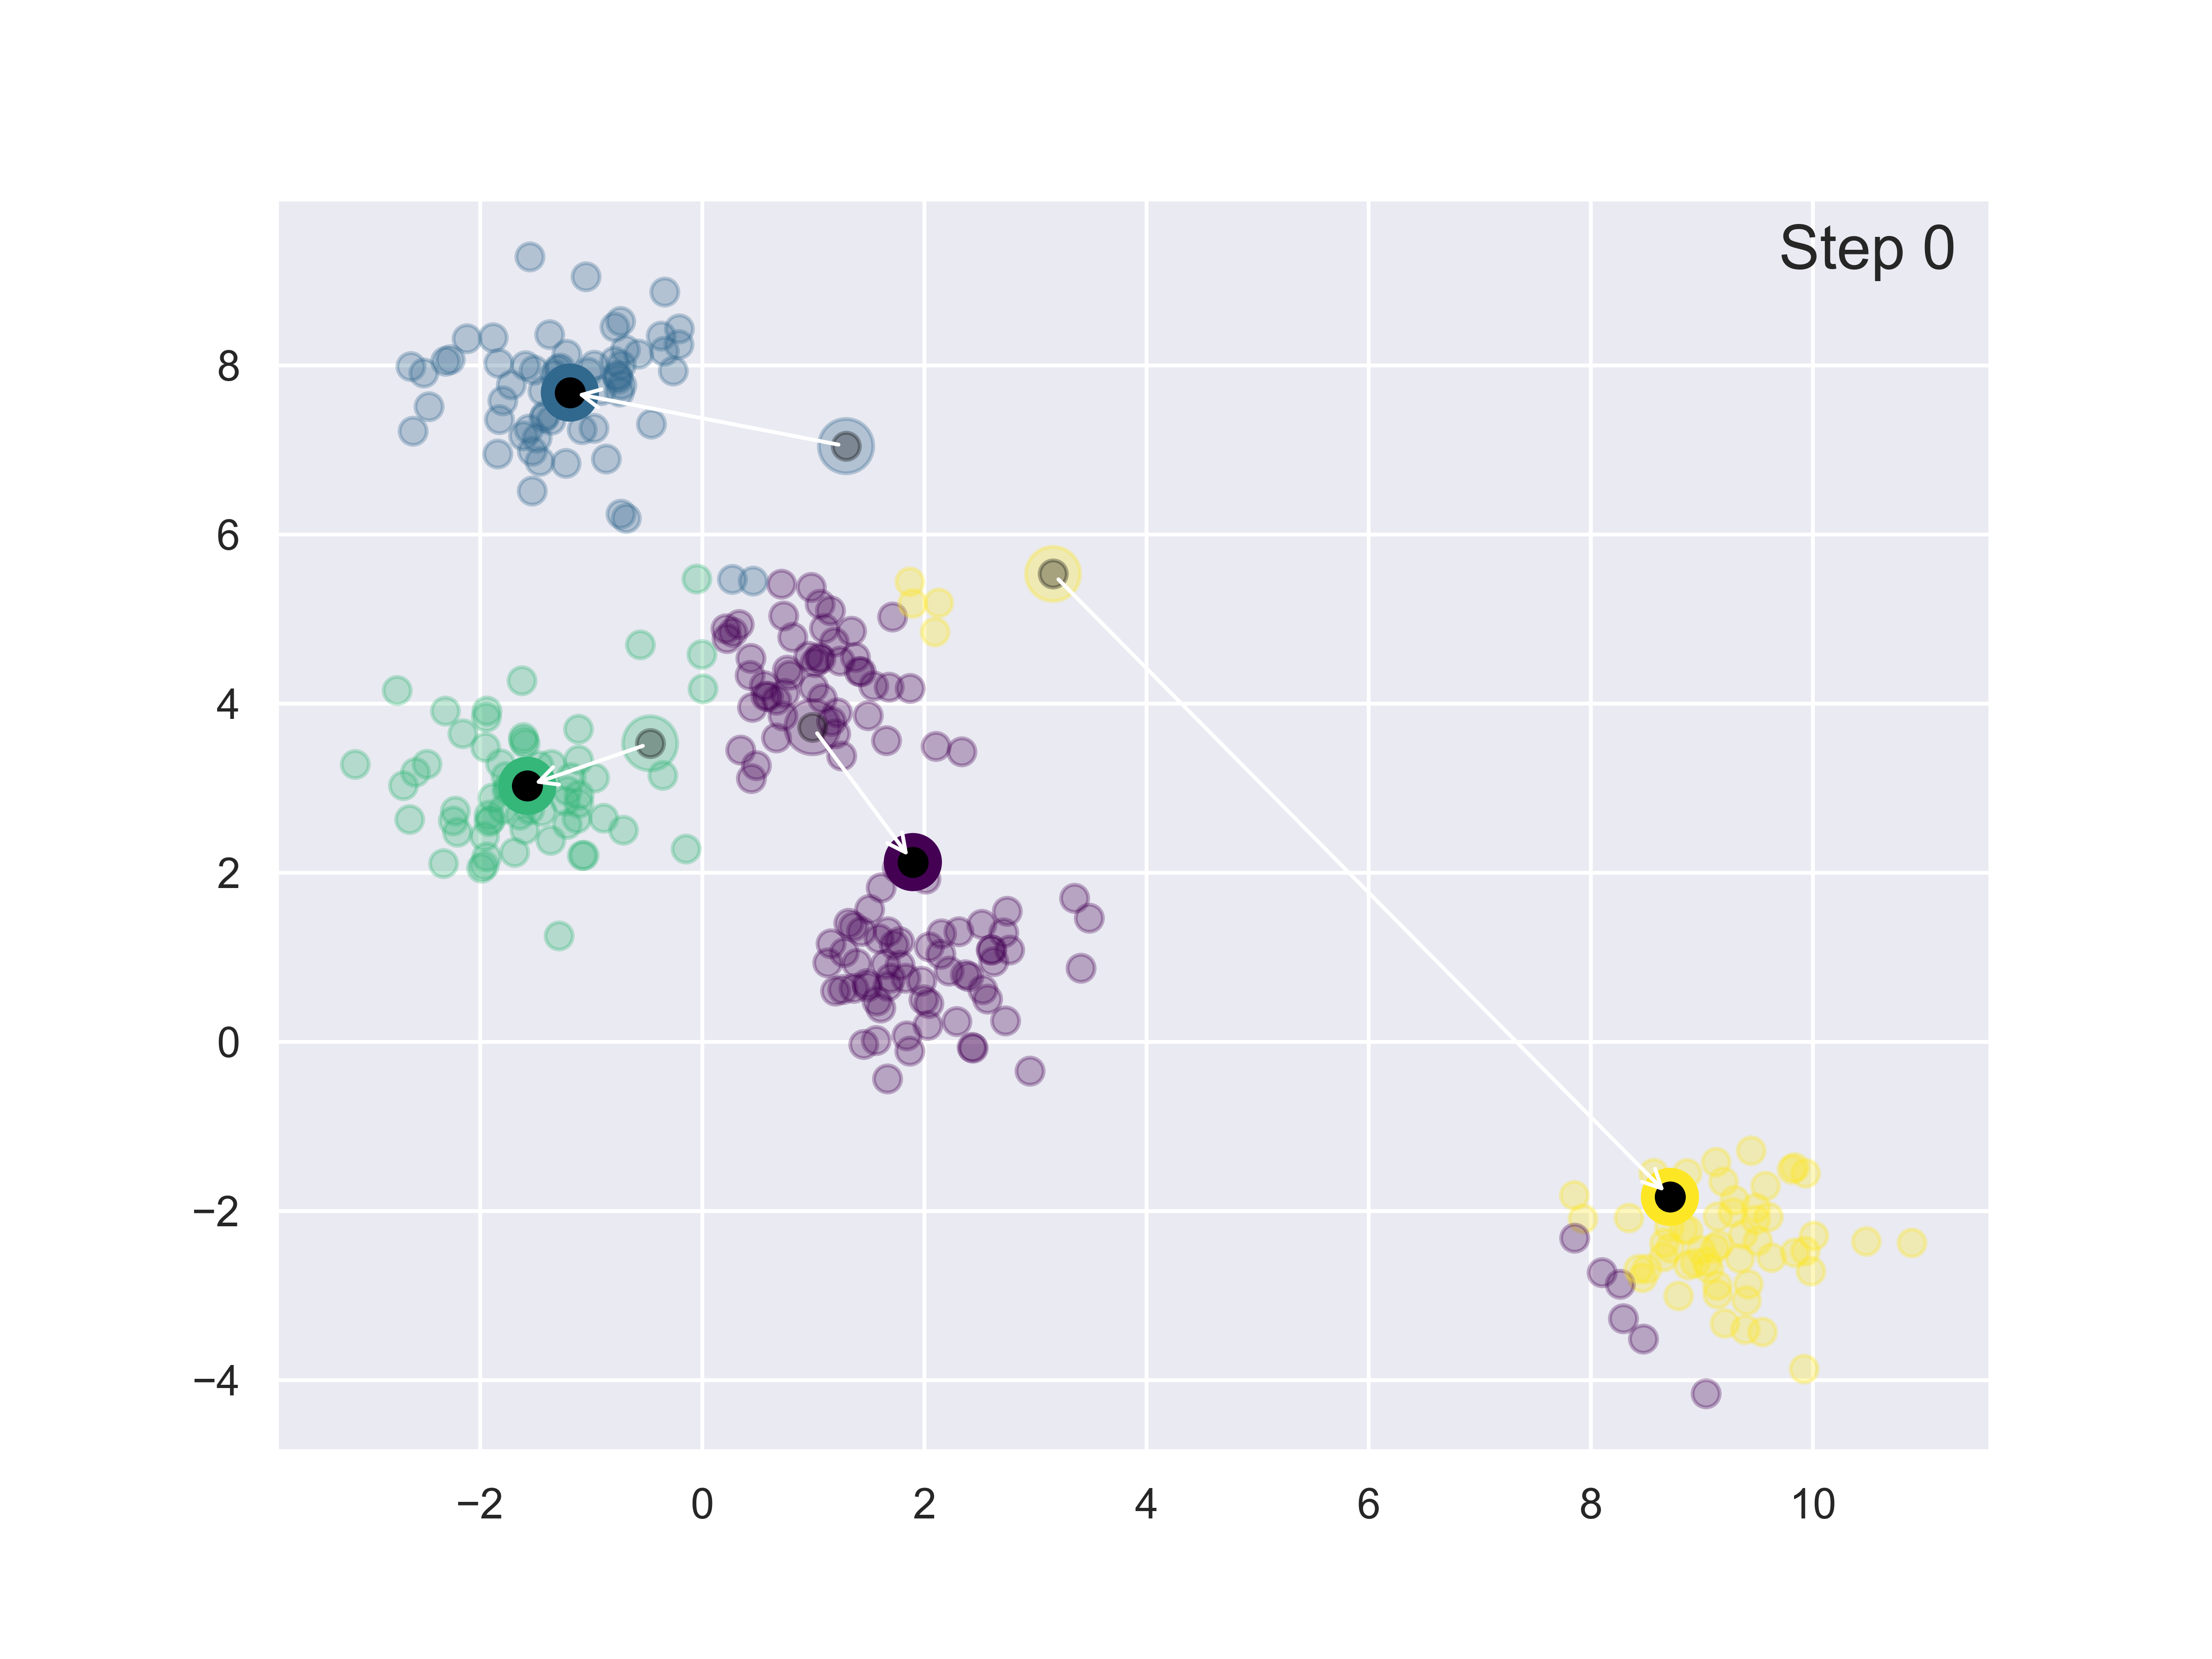
\includegraphics[width=0.7\textwidth]{PCAprocedureFewCluster1}\source{}}
			\only<3>{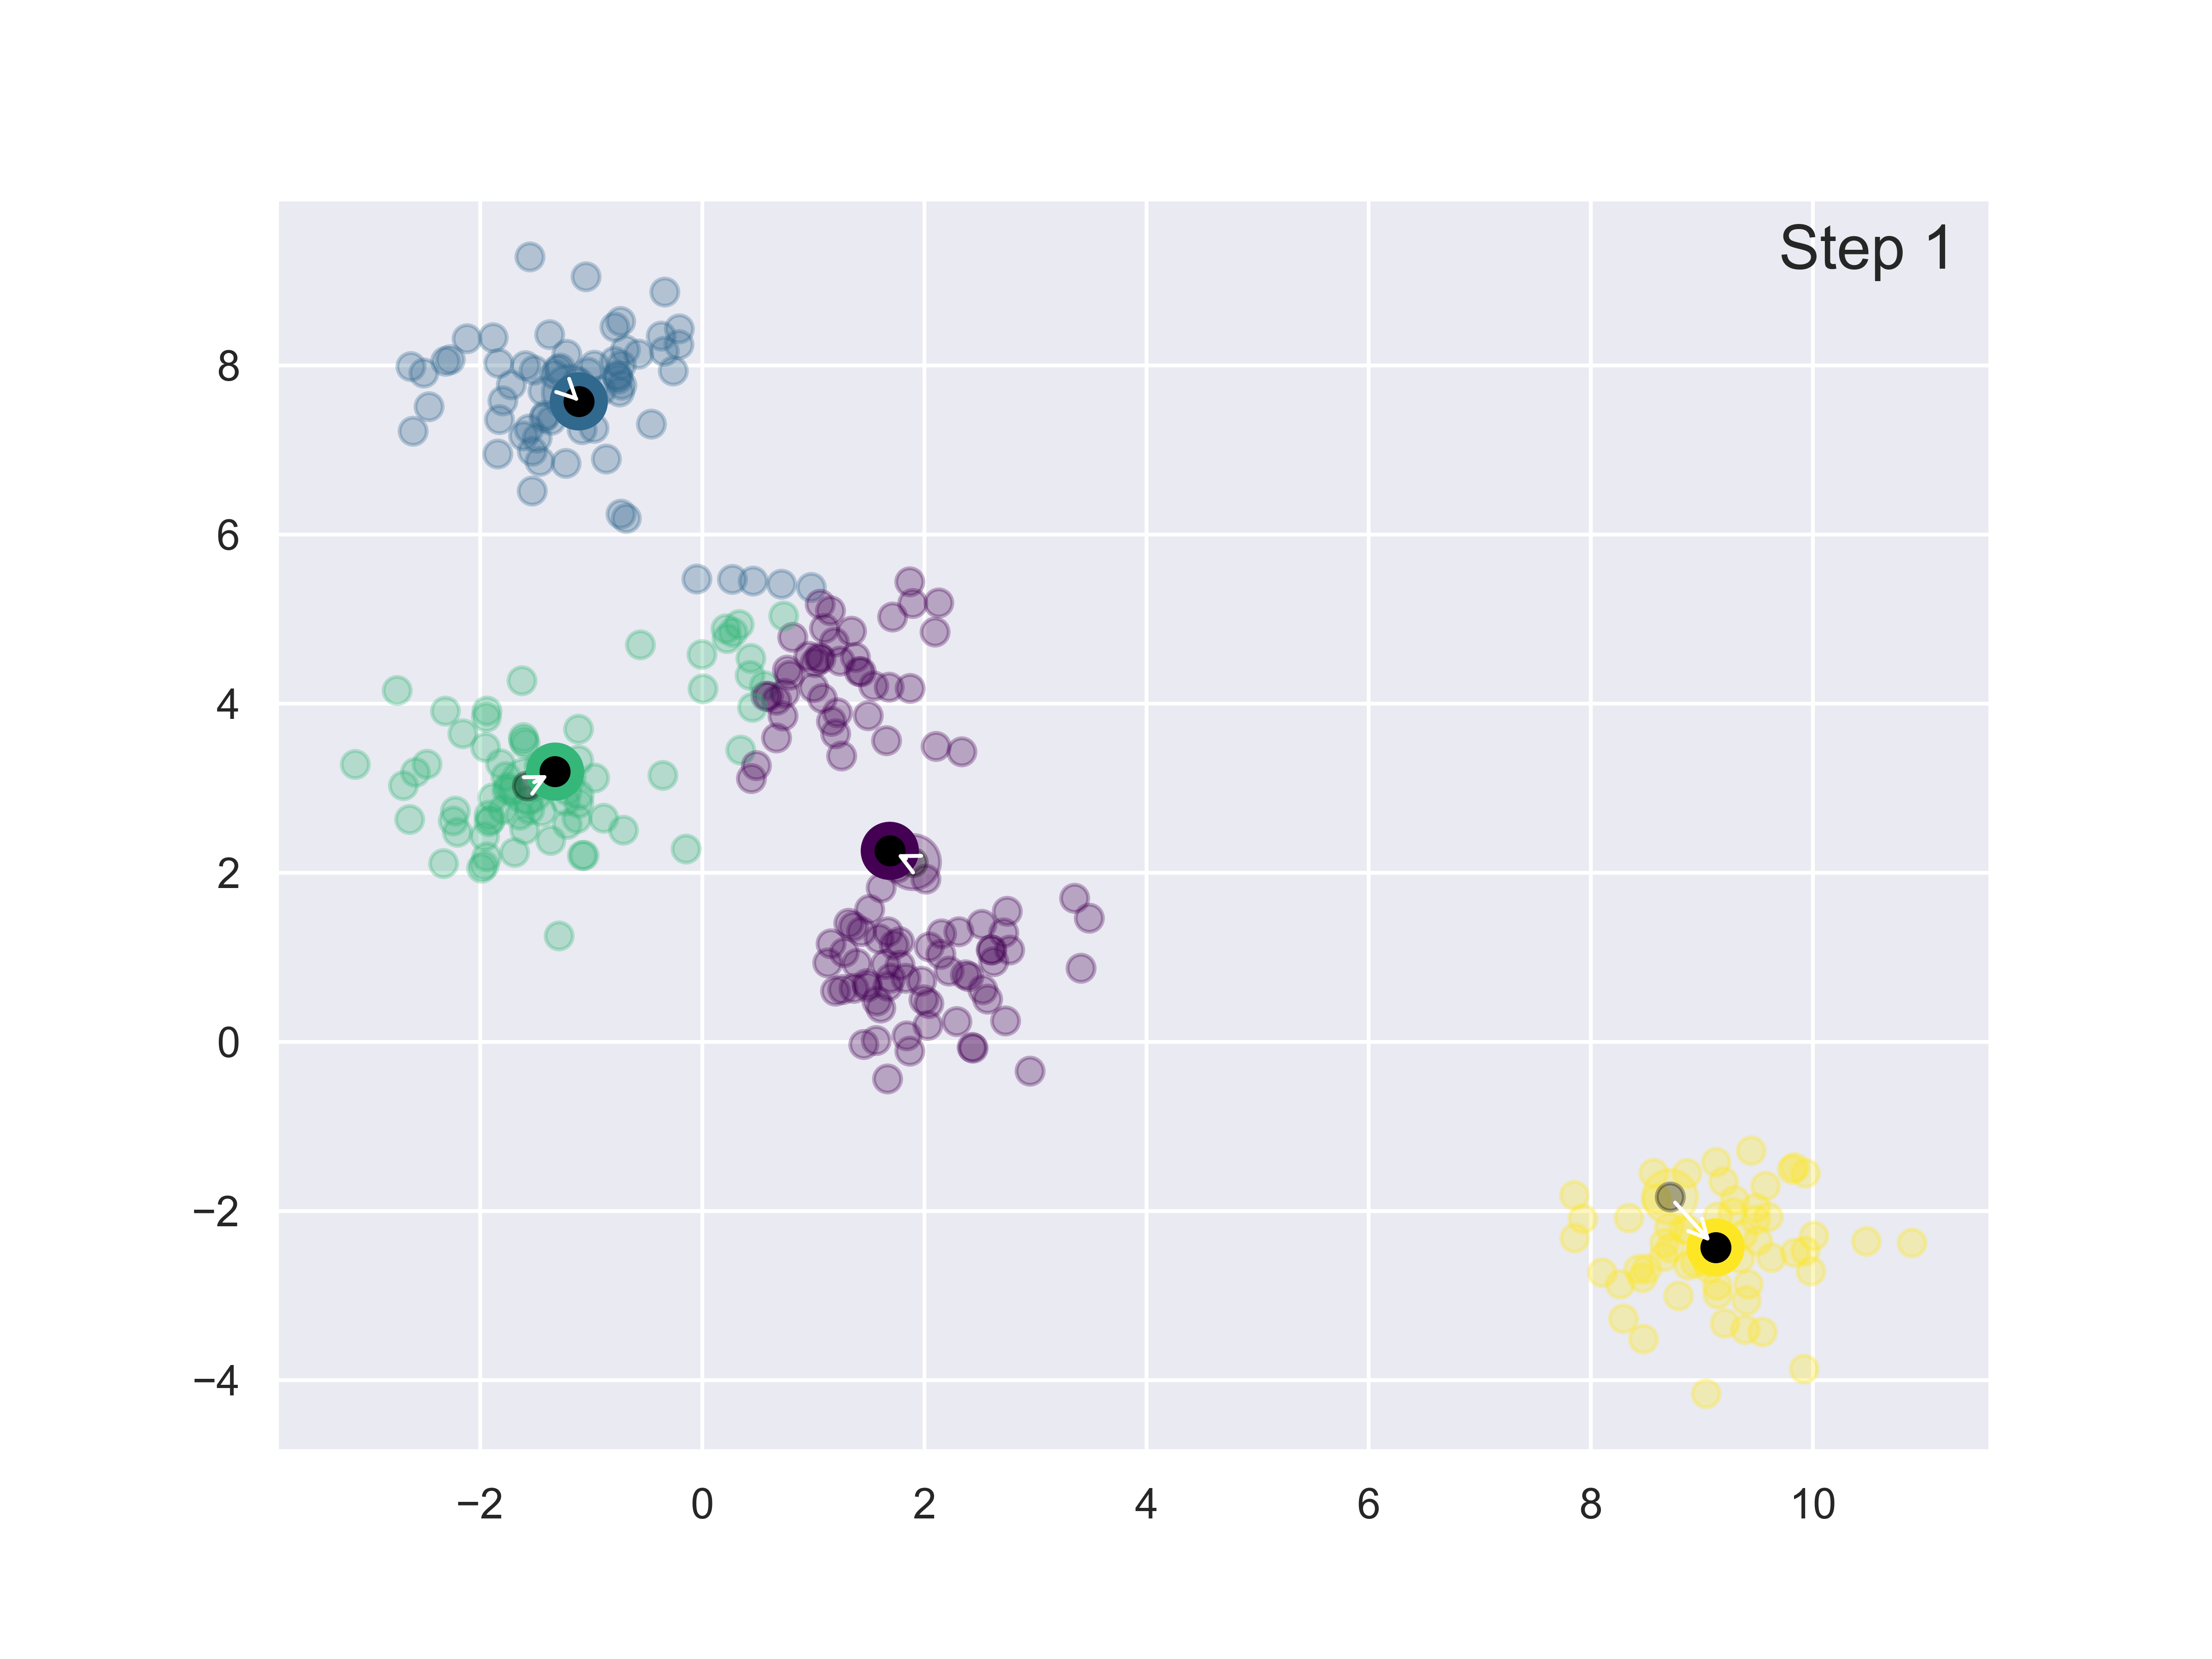
\includegraphics[width=0.7\textwidth]{PCAprocedureFewCluster2}\source{}}
			\only<4>{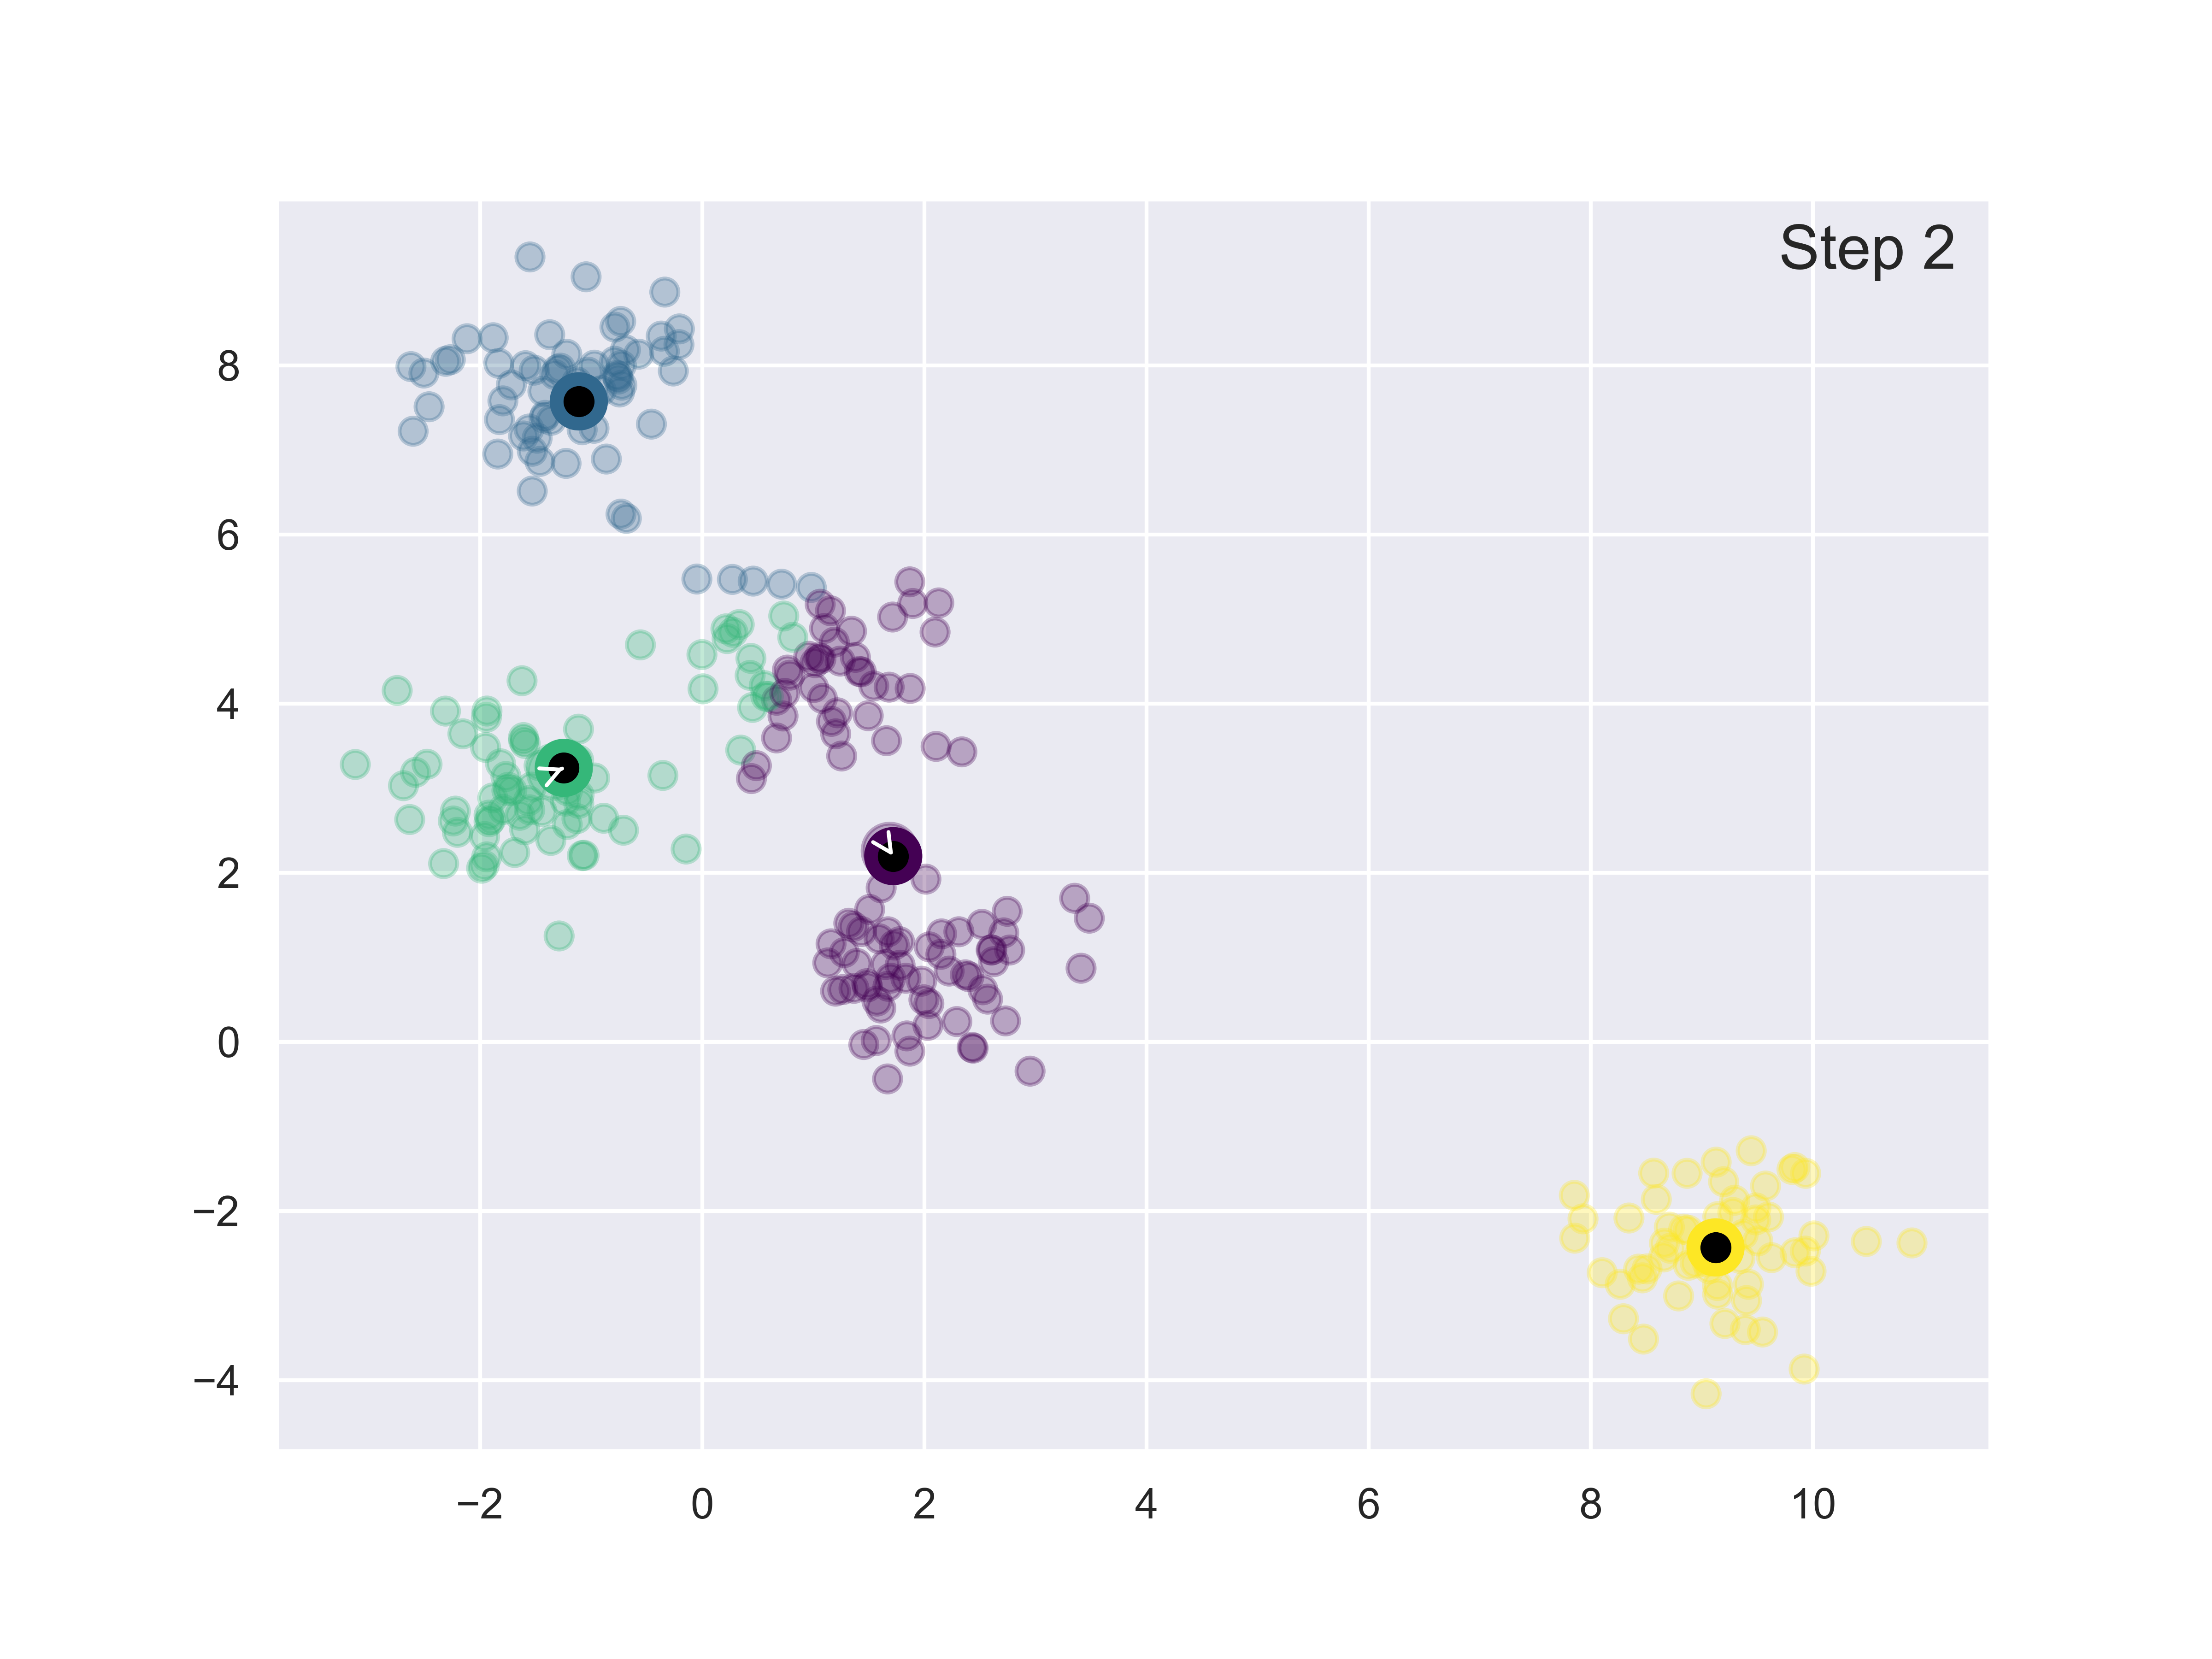
\includegraphics[width=0.7\textwidth]{PCAprocedureFewCluster3}\source{}}
			\only<5>{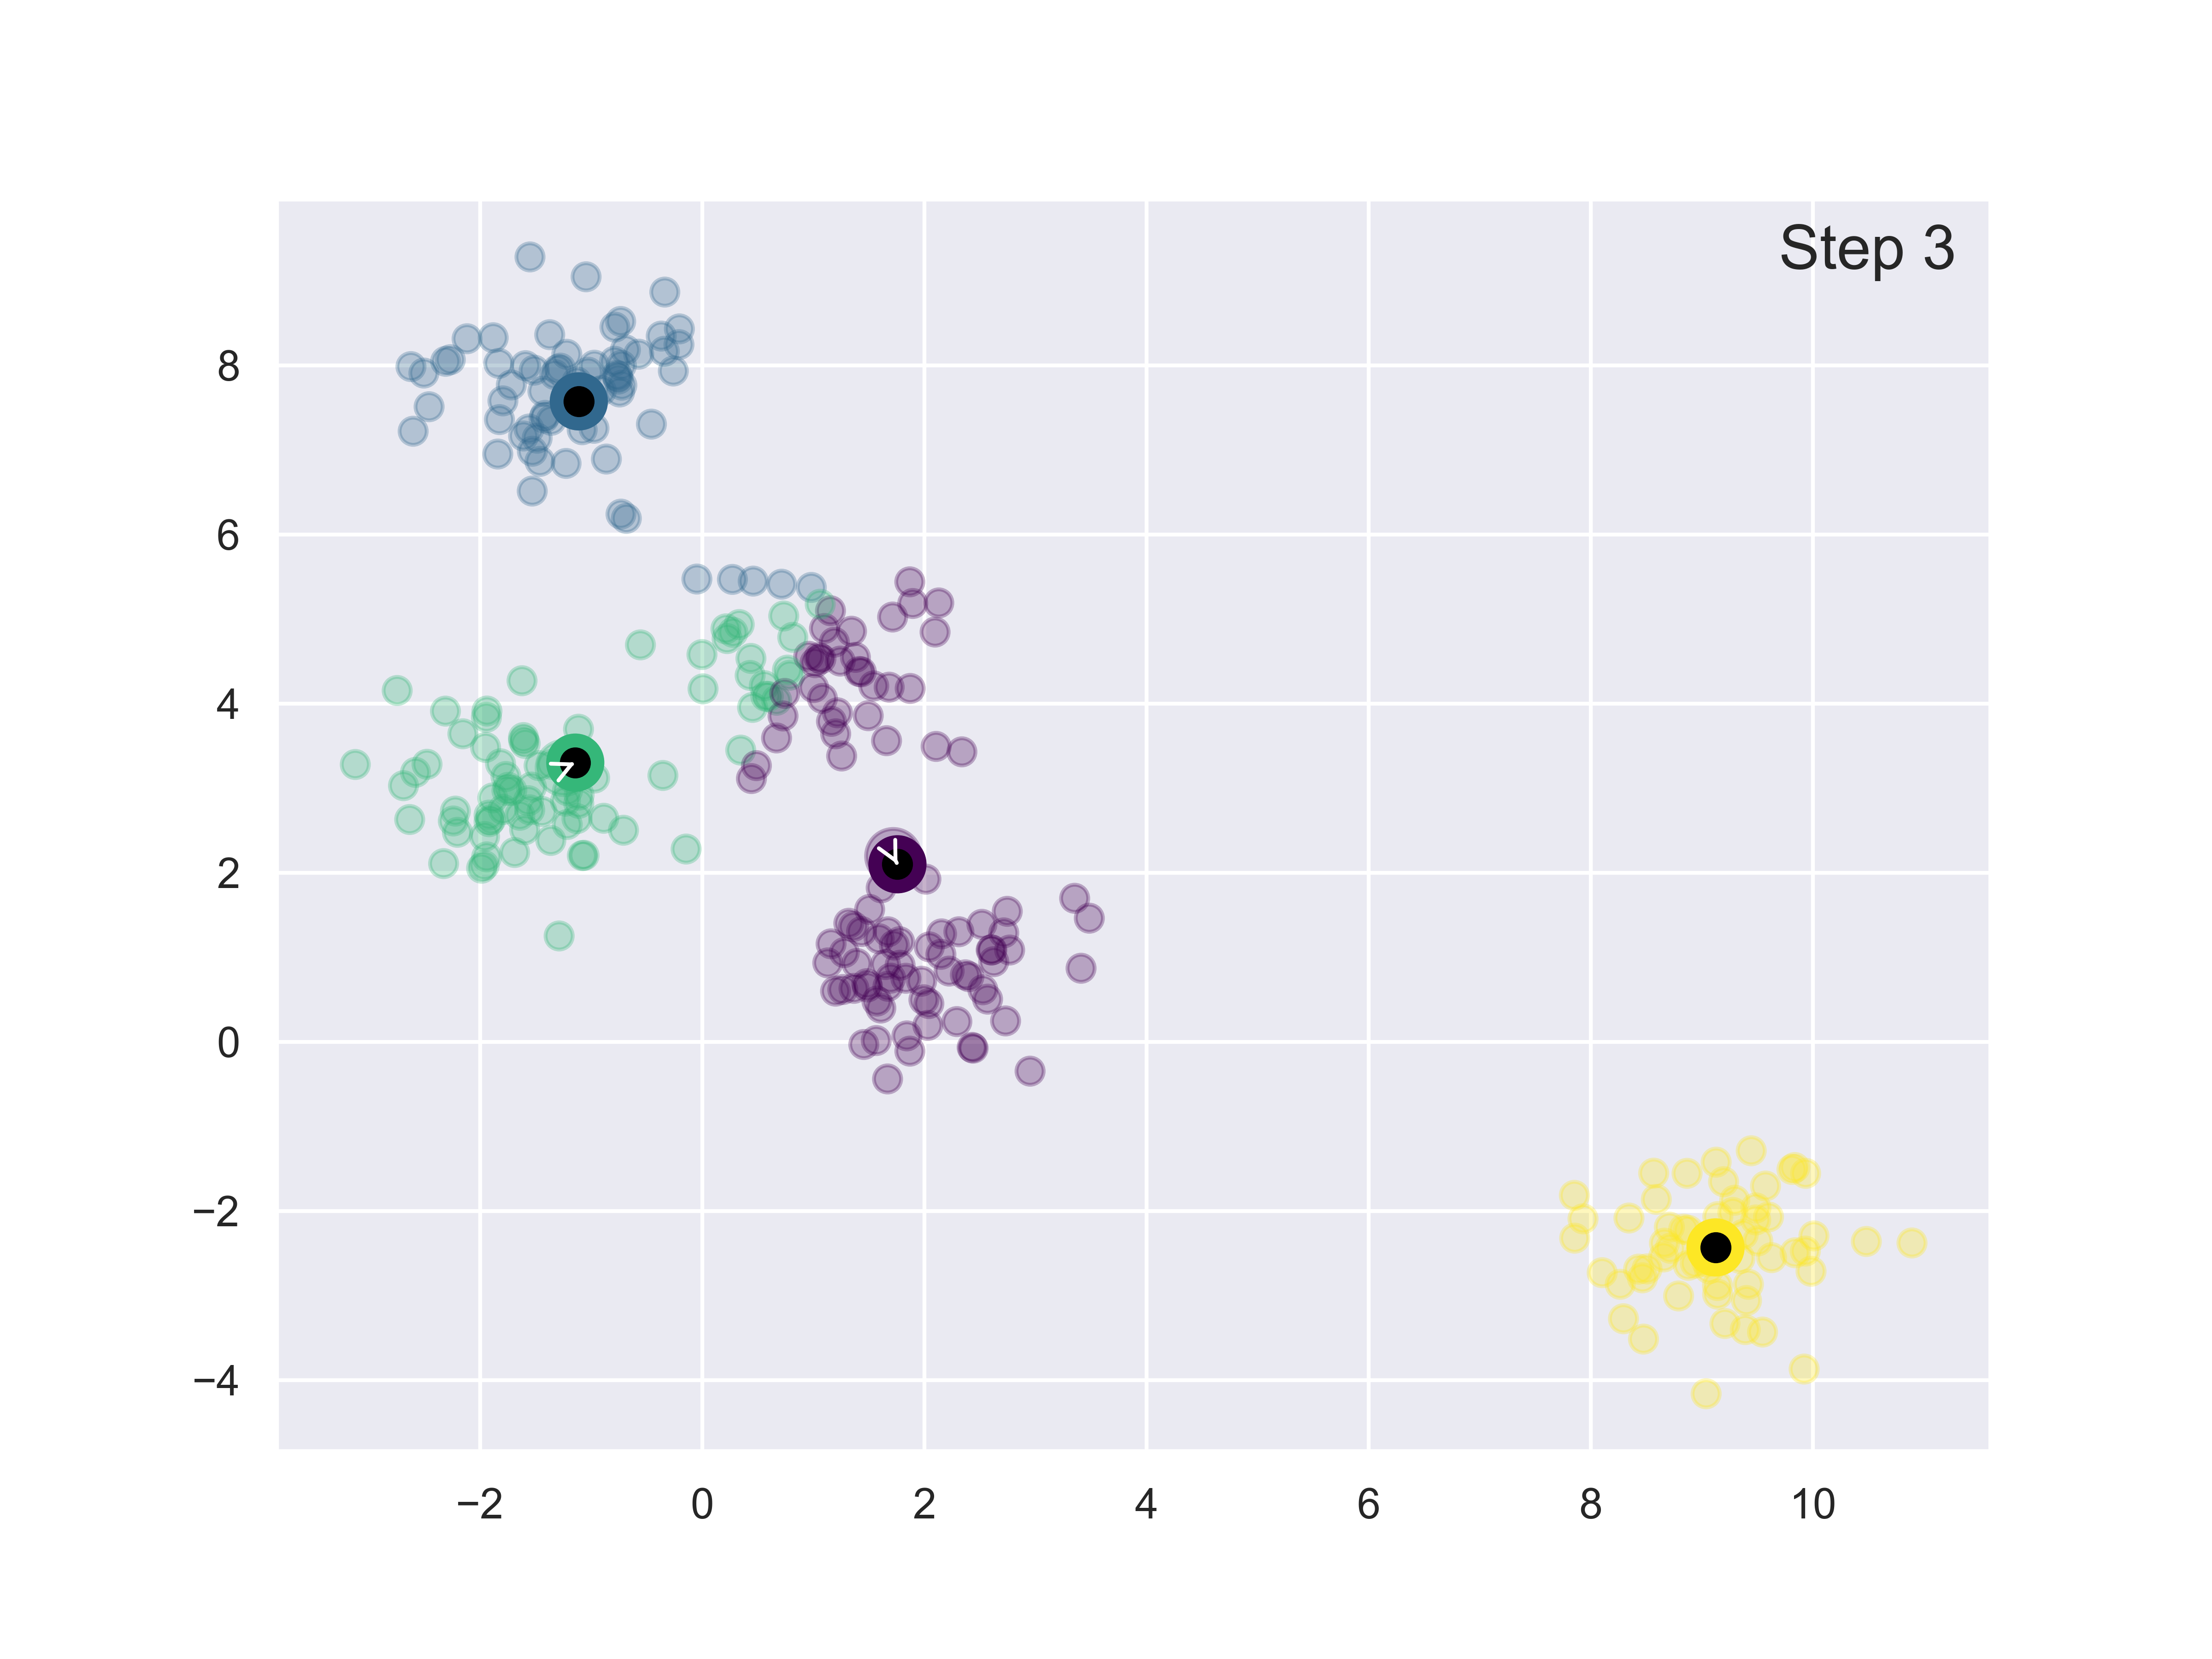
\includegraphics[width=0.7\textwidth]{PCAprocedureFewCluster4}\source{}}
			\only<6>{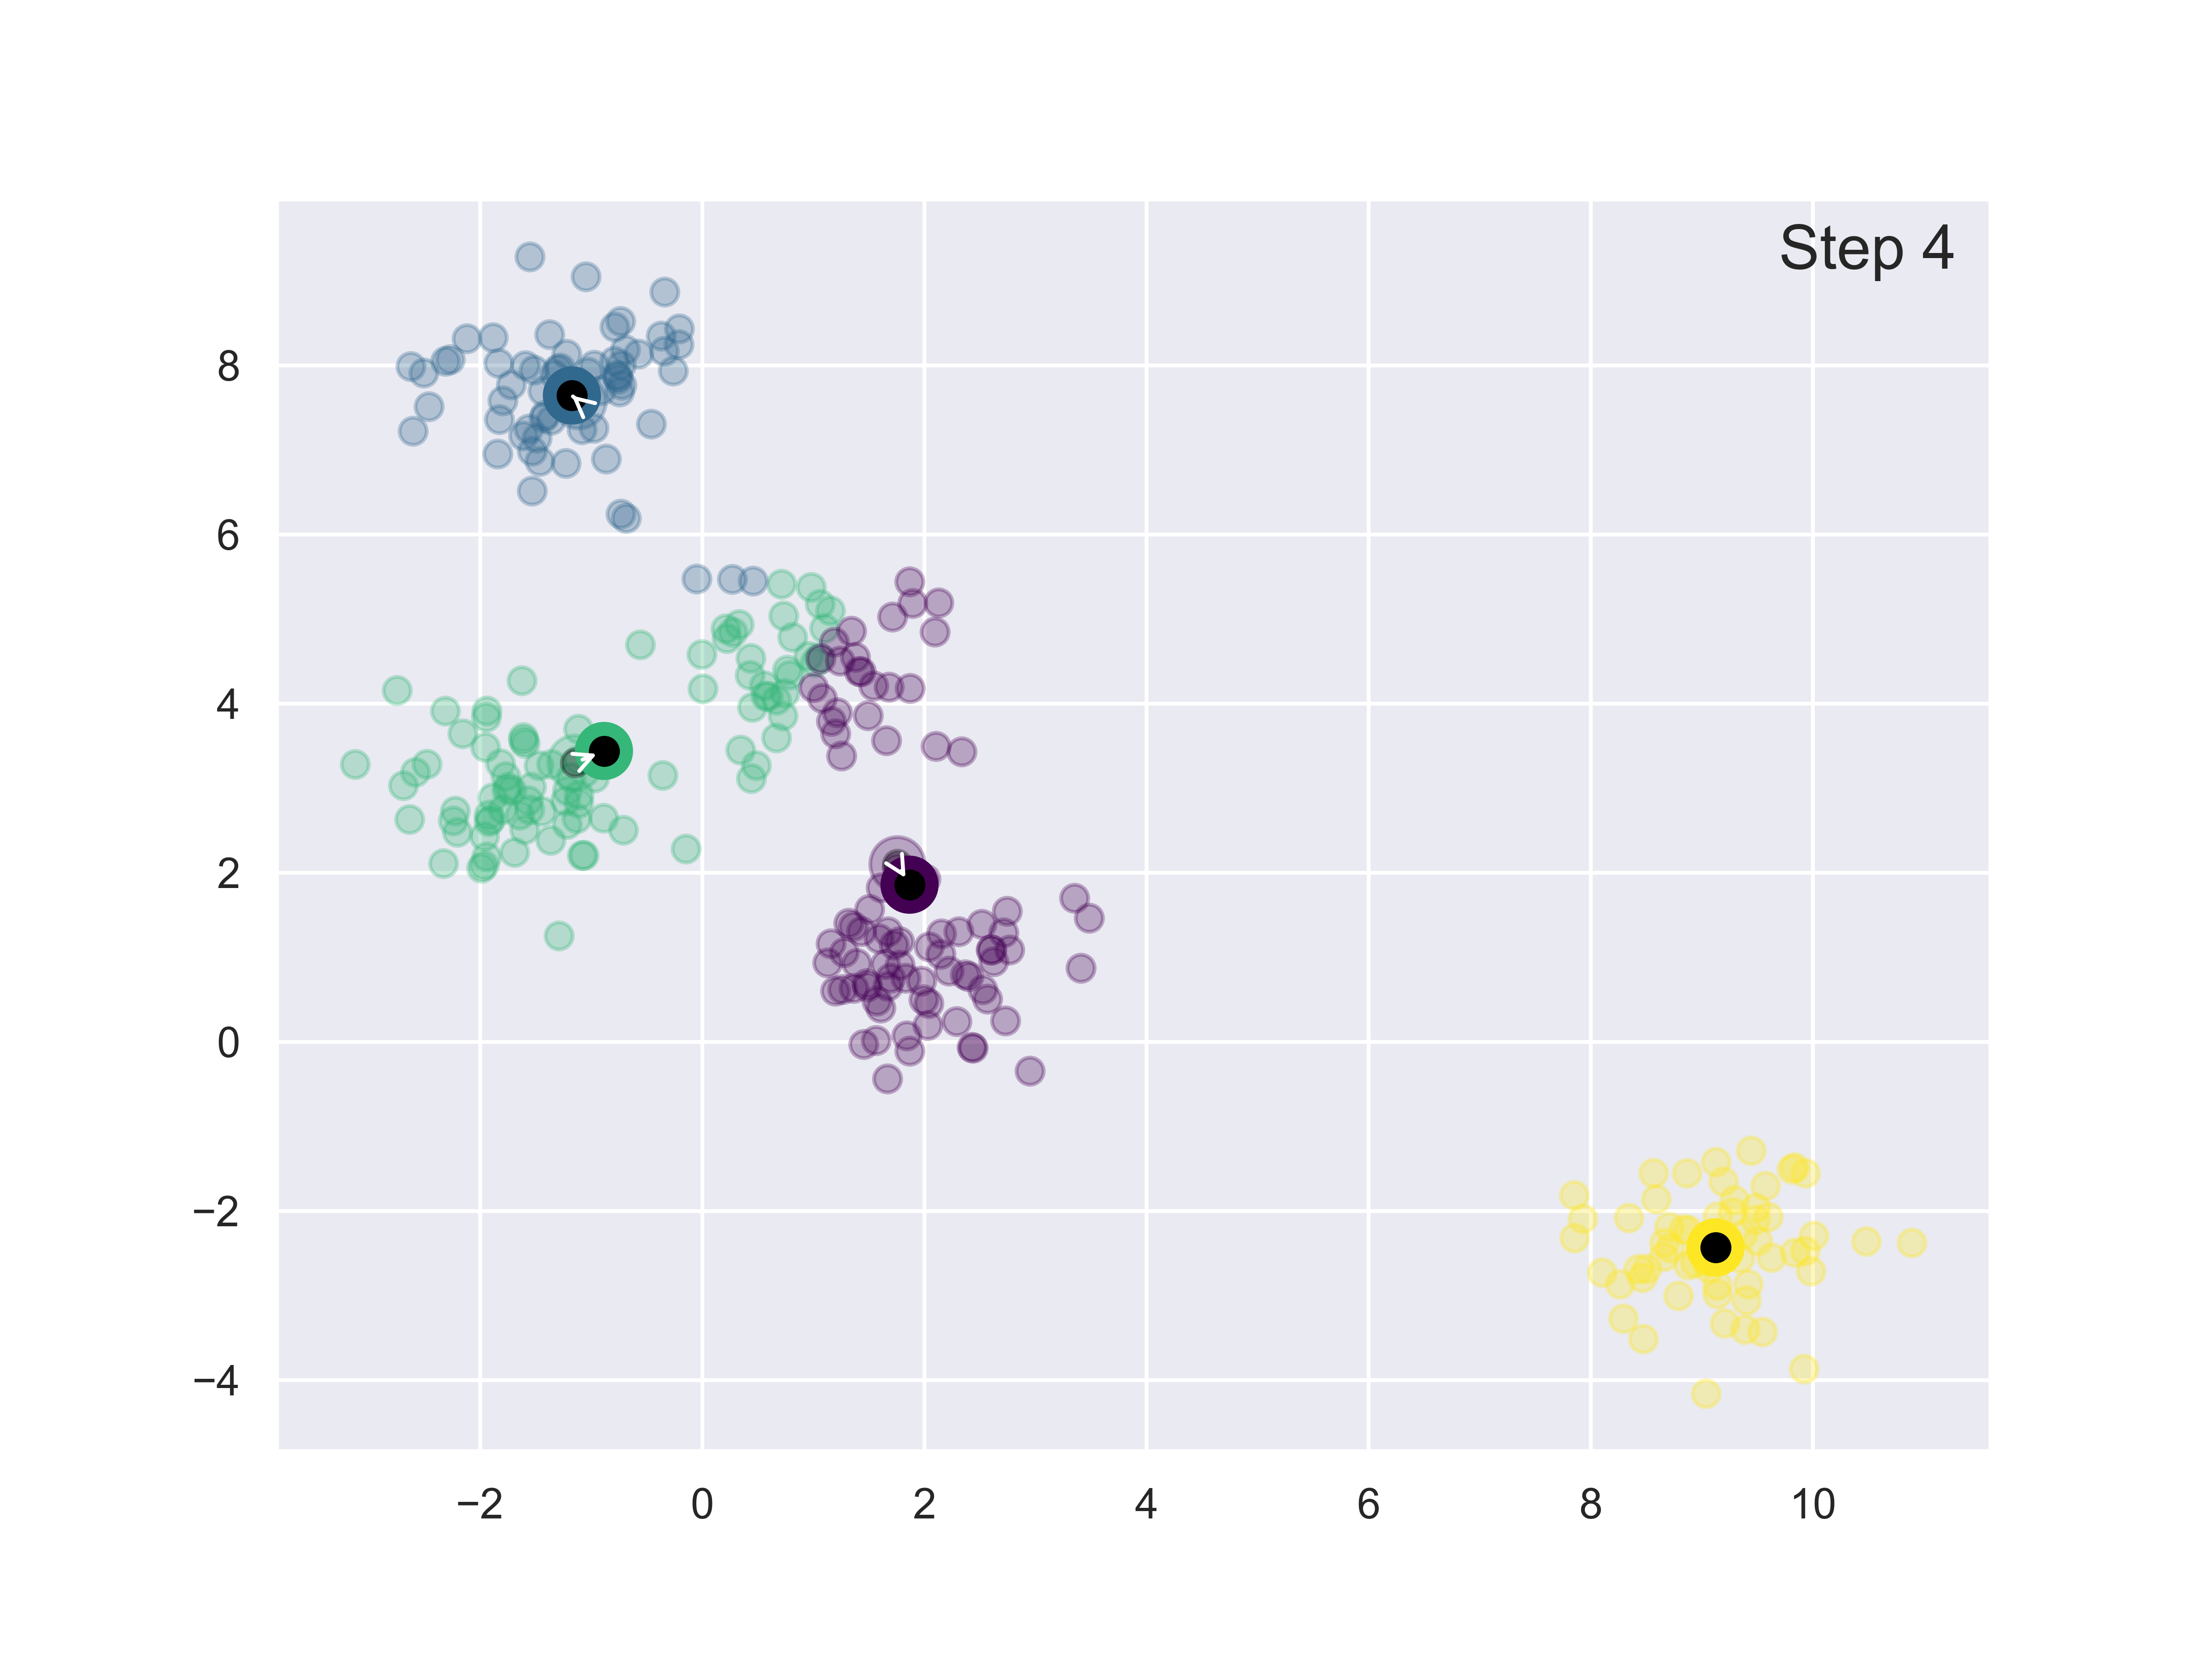
\includegraphics[width=0.7\textwidth]{PCAprocedureFewCluster5}\source{}}
			%\only<7>{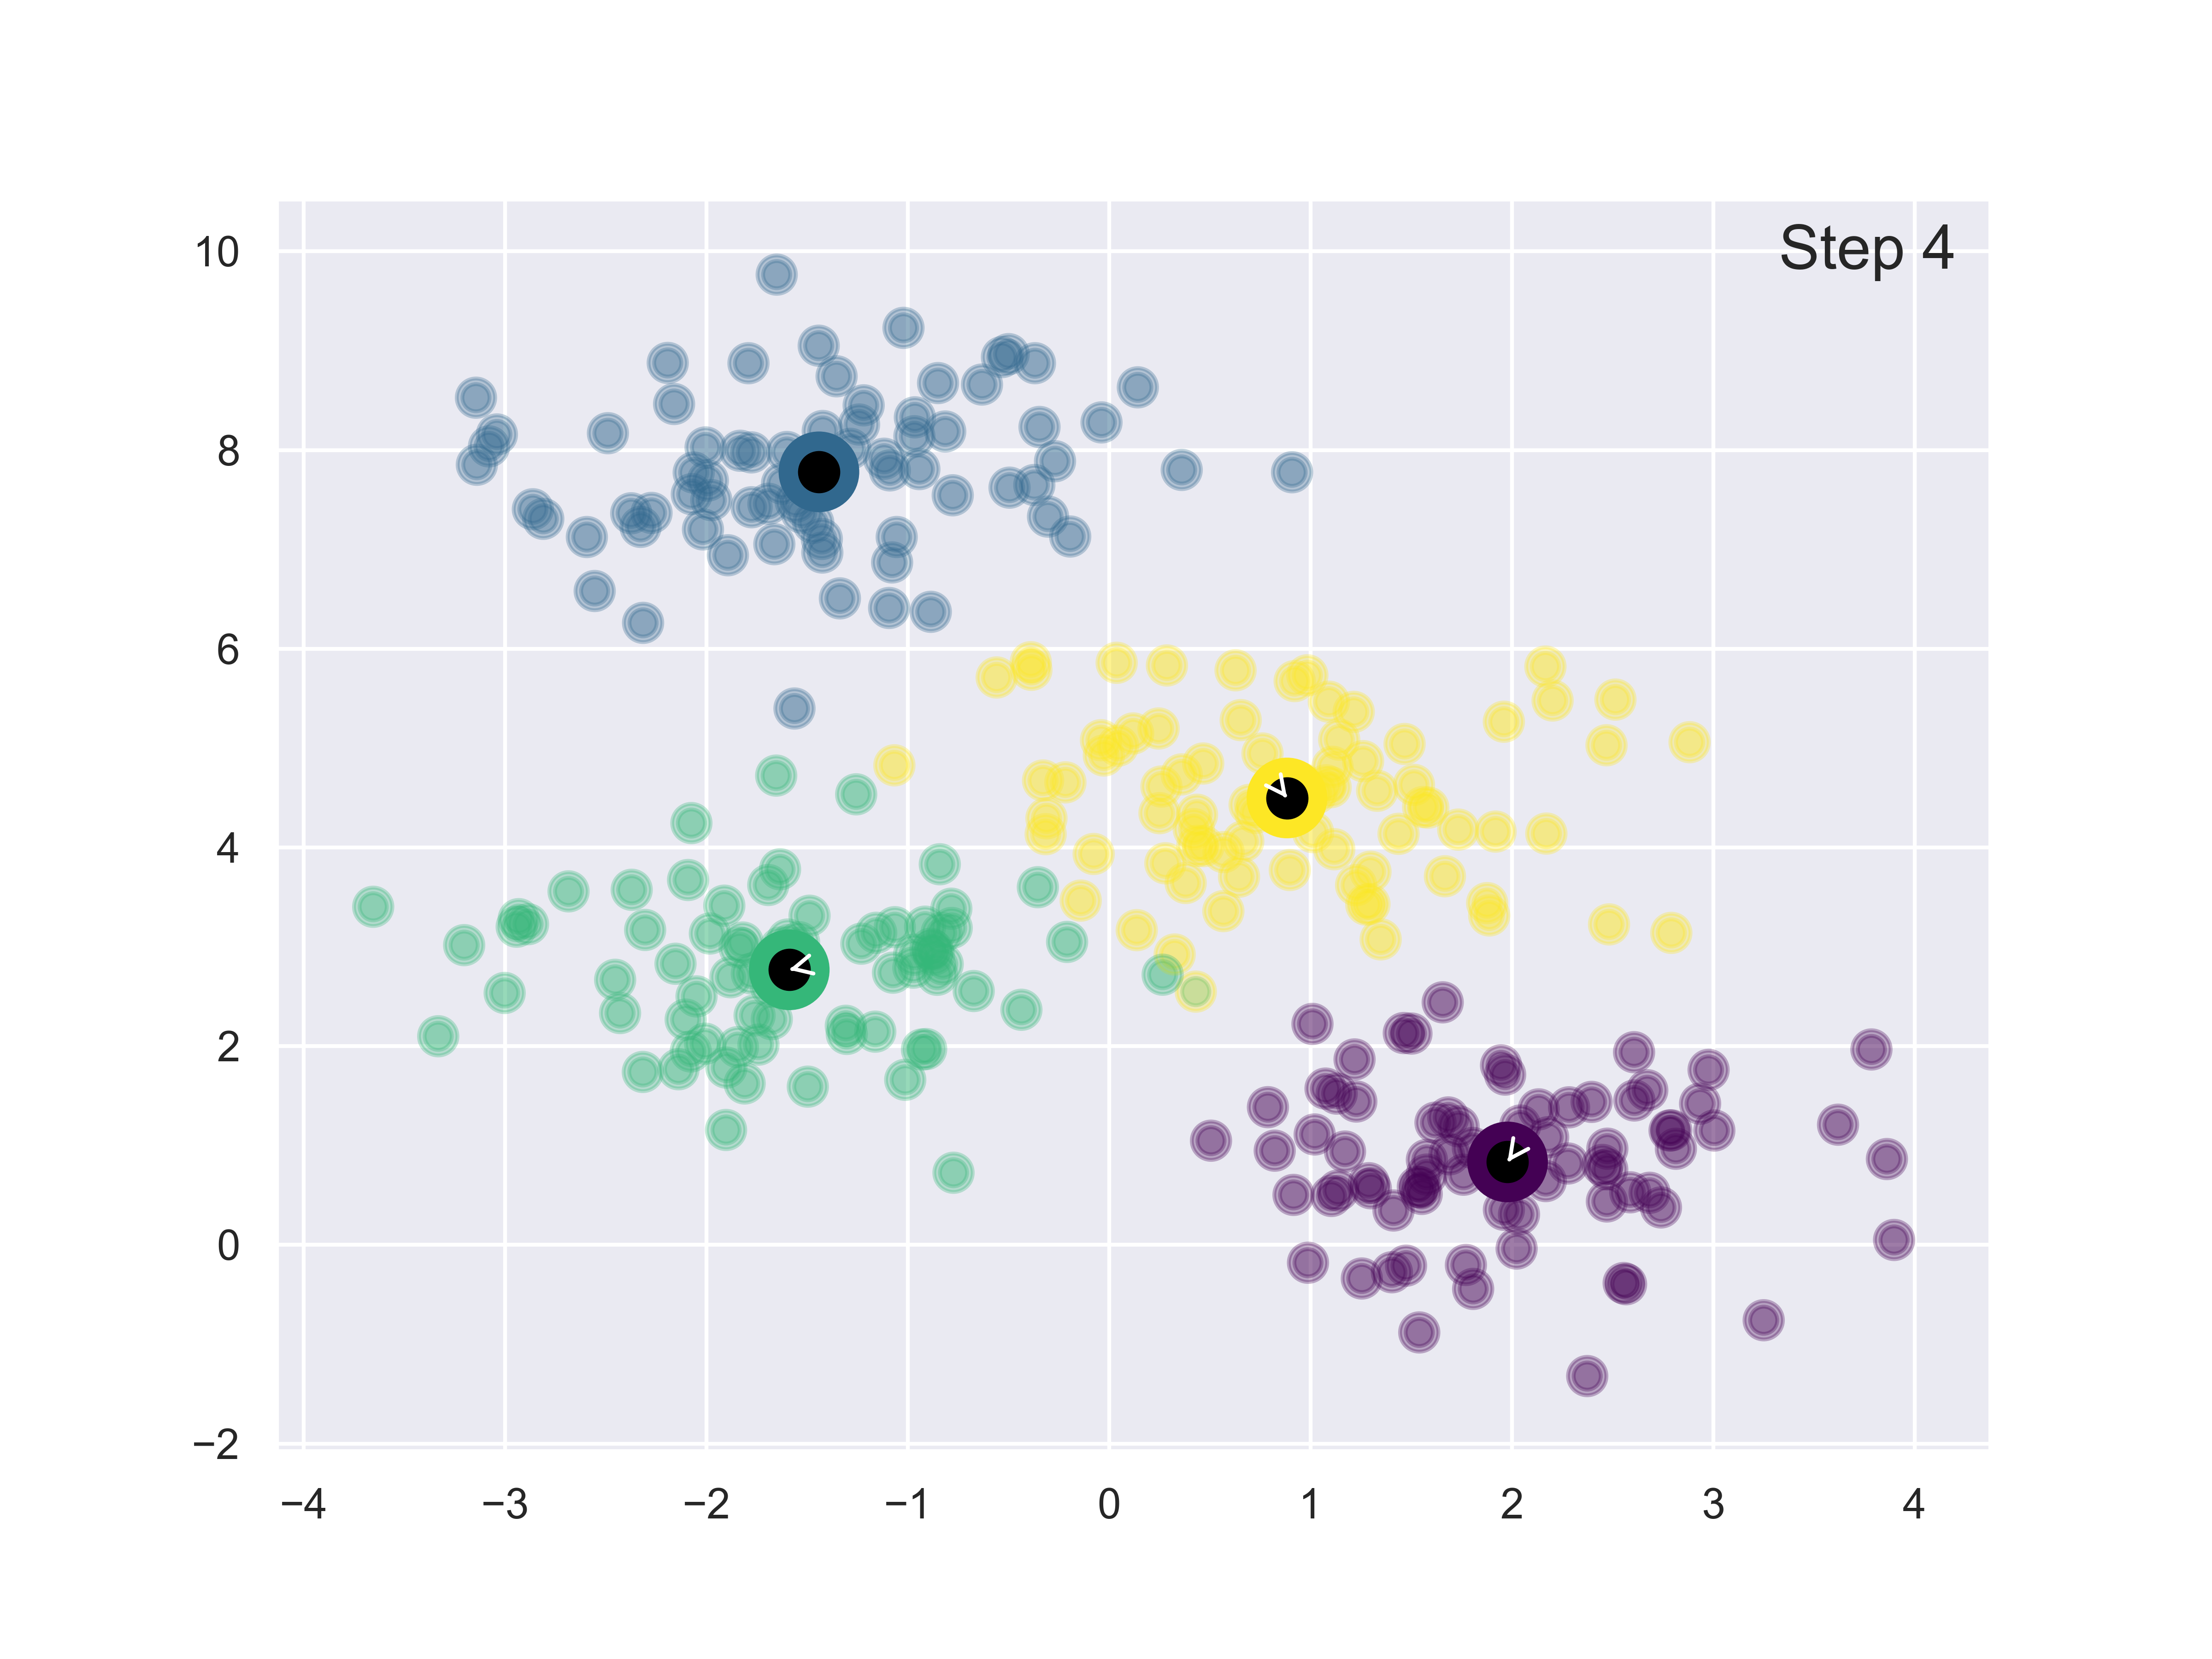
\includegraphics[width=0.7\textwidth]{PCAprocedure6}\source{}}

        		\end{center}}



\subsection{Principal Component Analysis}
%\frame{\frametitle{Principal Component Analysis (PCA)}
%\framesubtitle{Using MIT OpenCourseware Slides}
%Source:
%\begin{center}
%Philippe Rigollet. 18.650 Statistics for Applications . Fall 2016. Massachusetts Institute of Technology: MIT OpenCourseWare, https://ocw.mit.edu. License: Creative Commons BY-NC-SA.
%\end{center}
%}
%
%\setbeamercolor{background canvas}{bg=}
%%\frame{
%\includepdf[page = 2-16]{OCW/PCA.pdf}%}

\frame{\frametitle{Principal Component Analysis (PCA)}
\framesubtitle{Reduce dimensionality of data}
\begin{columns}[t] 
     \begin{column}[T]{7cm} 
     	\begin{itemize}
     		\item Sample $X_{1}, \ldots, X_{n}$ is a cloud of points in $\mathbb{R}^d$
		\item Typically, $d$ is large
		\item<1-> \textbf{Question:} can we project the point cloud onto a linear subspace of dimension $d' < d$ while keeping as much of the information as possible?
		\item<2-> \textbf{Answer:} PCA achieves this by keeping important aspects of the covariance structure in orthogonal directions.
     	\end{itemize}
     \end{column}
     	\begin{column}[T]{7cm} 
         	\begin{center}
            		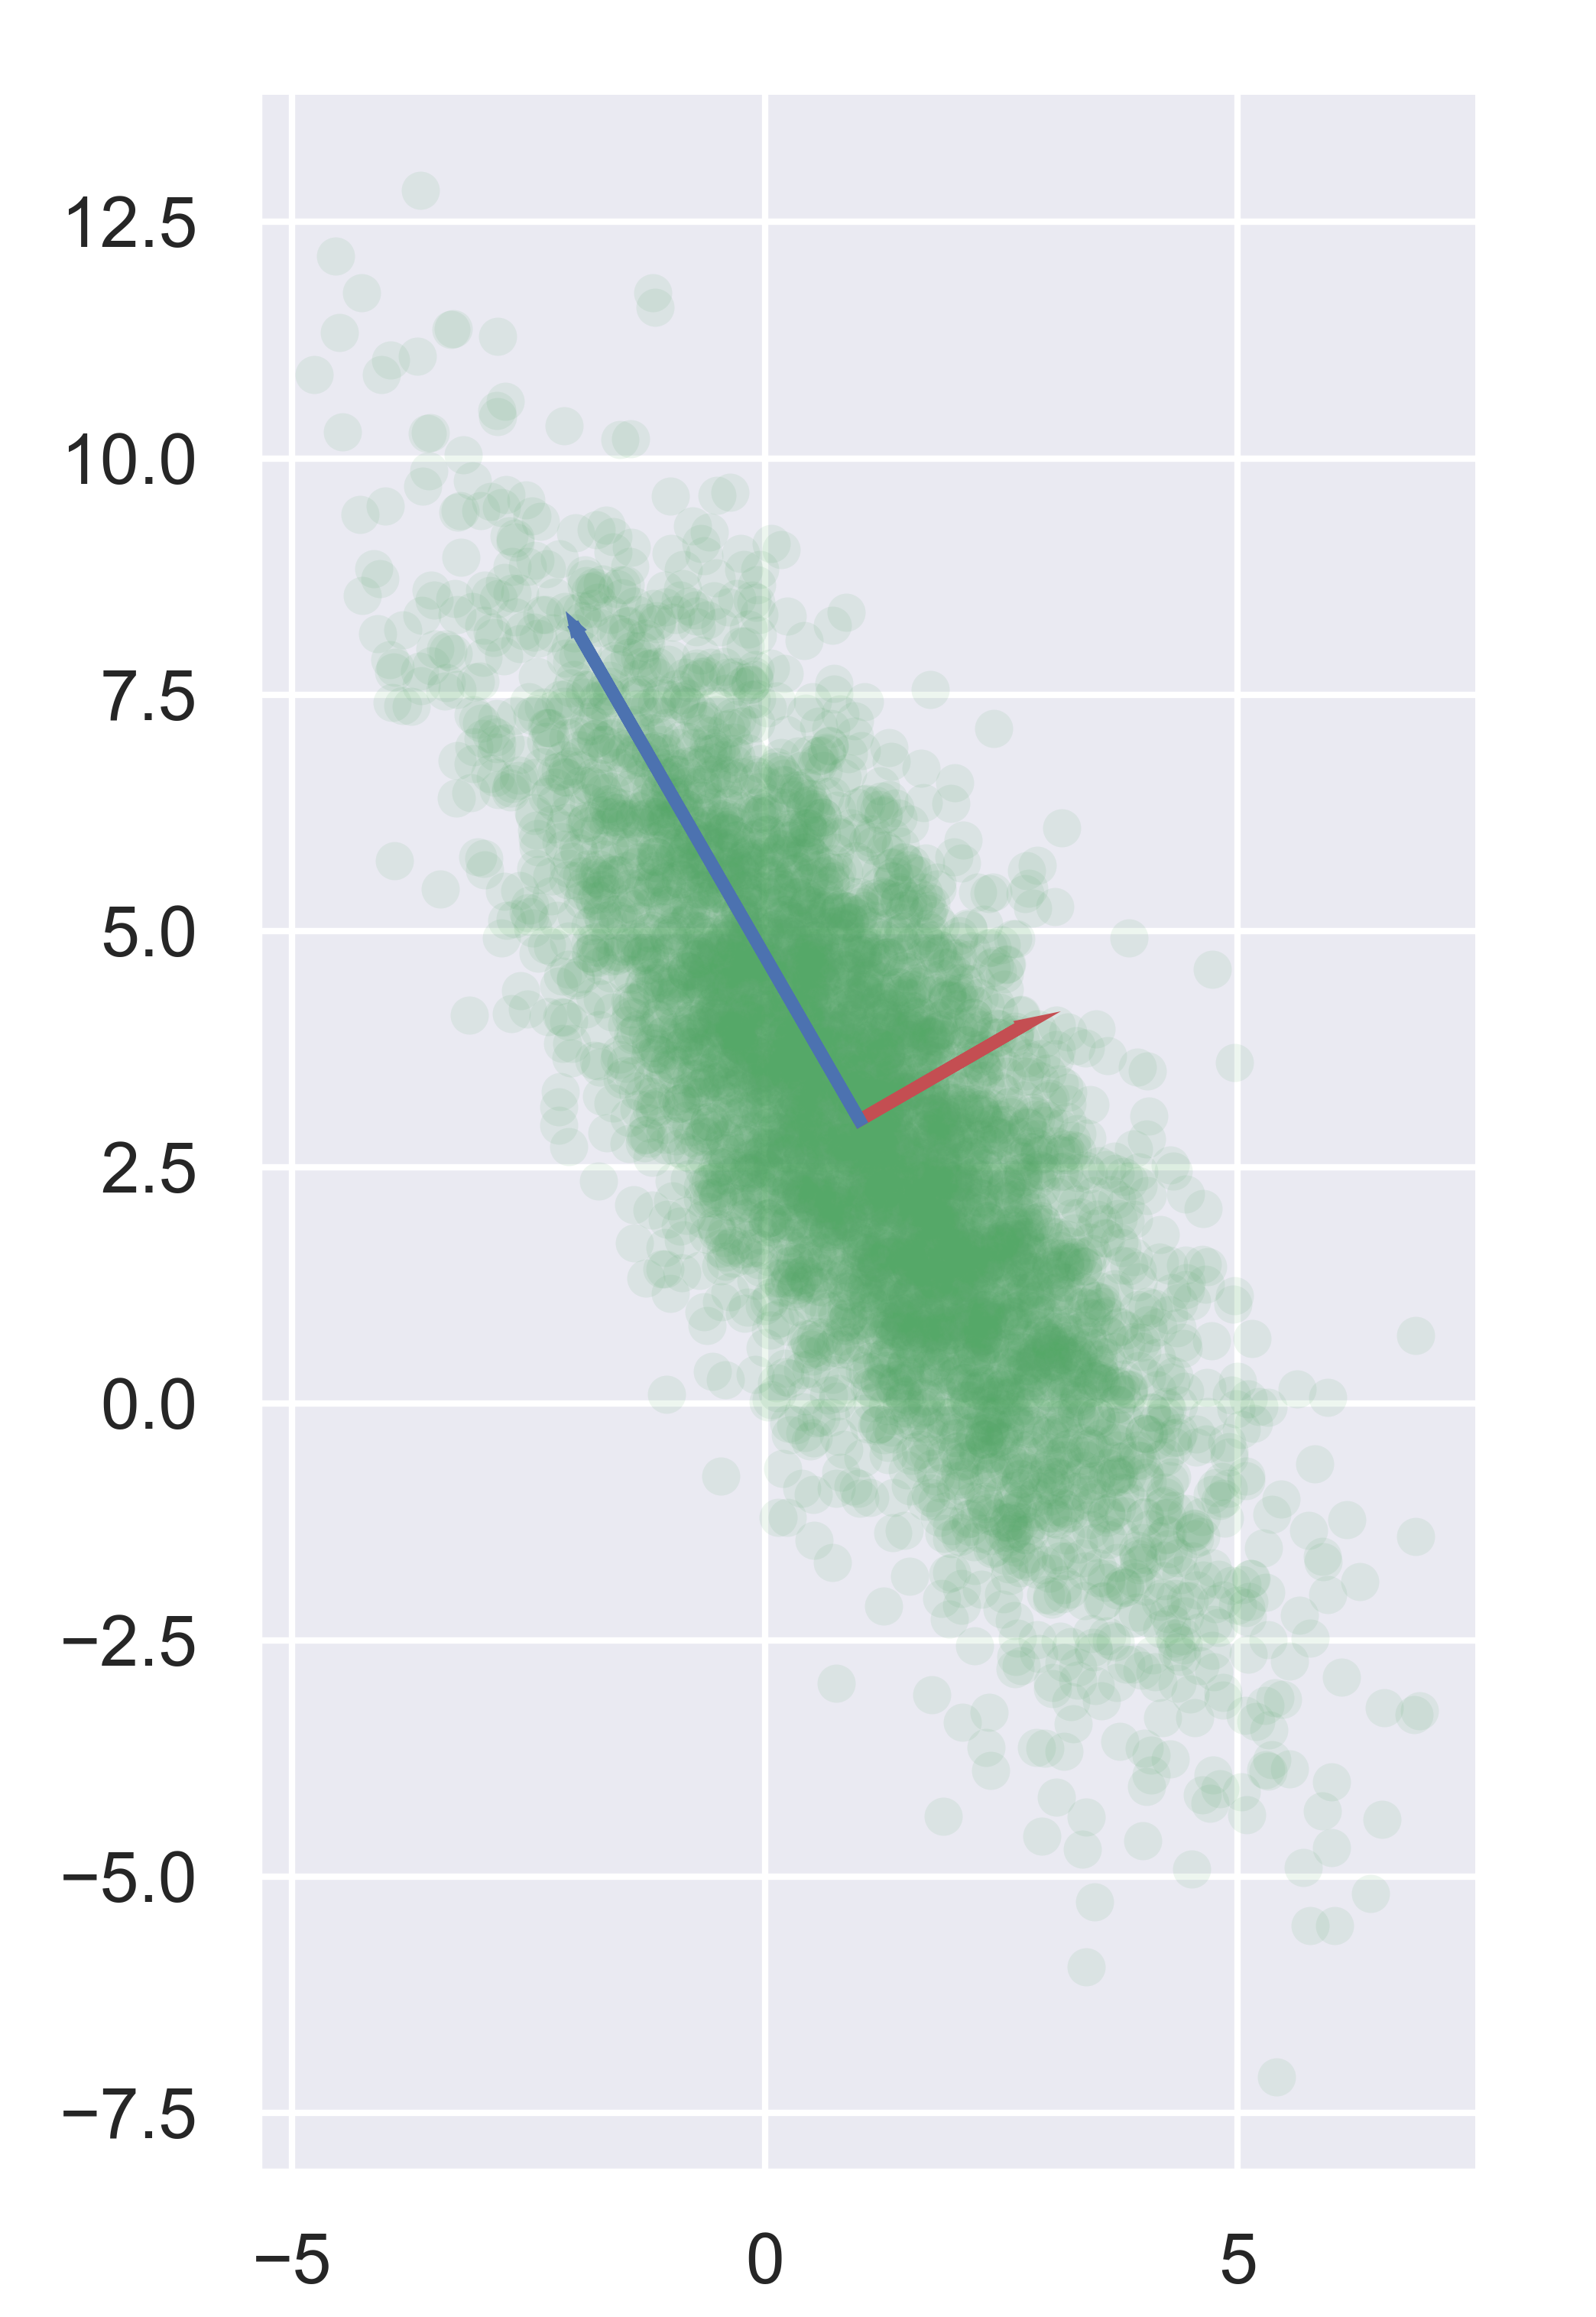
\includegraphics[width=0.6\textwidth]{GaussianScatterPCA}\source{}
        		\end{center}
     \end{column}
 \end{columns}
}



\subsection{Support Vector Machines}

\frame{\frametitle{Support Vector Machine}
\framesubtitle{Separate data into subsets according to their $nD$-coordinates.}
\begin{columns}[t] 
     \begin{column}[T]{7cm} 
     	\begin{itemize}
		\item Idea:
		\begin{itemize}
		\item Find separating hyperplane maximising the distance between borderline instances
		\item For data mixed in feature space, slack parameter (and penalty $C$) is used
		\item If no separating hyperplane can be found in feature space, dimension is increased ``Kernel trick''
		\end{itemize}
     		\item Robust:
		\begin{itemize}
		\item High dimensionality
		\item Small datasets
		\end{itemize}
		\item Simple to complex models
     	\end{itemize}
     \end{column}
     	\begin{column}[T]{7cm} 
         	\begin{center}
		\only<1>{
            		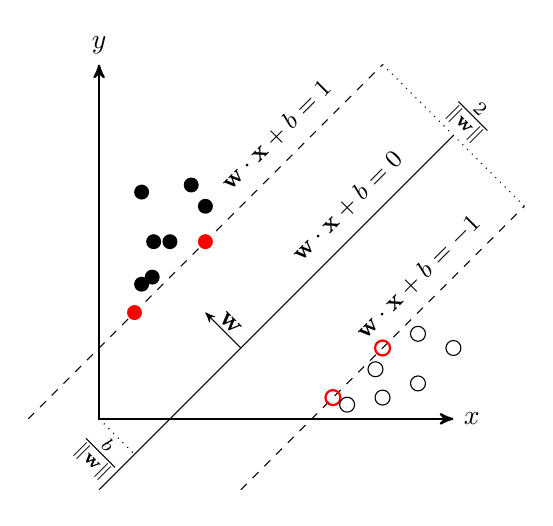
\begin{tikzpicture}[>=stealth', scale = 0.9]
                      % Draw axes
                      \draw [<->,thick] (0,5) node (yaxis) [above] {$y$}
                            |- (5,0) node (xaxis) [right] {$x$};
                      % draw line
                      \draw (0,-1) -- (5,4); % y=x-1
                      \draw[dashed] (-1,0) -- (4,5); % y=x+1
                      \draw[dashed] (2,-1) -- (6,3); % y=x-3
                      % \draw labels
                      \draw (3.5,3) node[rotate=45,font=\small] 
                            {$\mathbf{w}\cdot \mathbf{x} + b = 0$};
                      \draw (2.5,4) node[rotate=45,font=\small] 
                            {$\mathbf{w}\cdot \mathbf{x} + b = 1$};
                      \draw (4.5,2) node[rotate=45,font=\small] 
                            {$\mathbf{w}\cdot \mathbf{x} + b = -1$};
                      % draw distance
                      \draw[dotted] (4,5) -- (6,3);
                      \draw (5.25,4.25) node[rotate=-45] {$\frac{2}{\Vert \mathbf{w} \Vert}$};
                      \draw[dotted] (0,0) -- (0.5,-0.5);
                      \draw (0,-0.5) node[rotate=-45] {$\frac{b}{\Vert \mathbf{w} \Vert}$};
                      \draw[->] (2,1) -- (1.5,1.5);
                      \draw (1.85,1.35) node[rotate=-45] {$\mathbf{w}$};
                      % draw negative dots
                      \fill[red] (0.5,1.5) circle (3pt);
                      \fill[red]   (1.5,2.5)   circle (3pt);
                      \fill[black] (1,2.5)     circle (3pt);
                      \fill[black] (0.75,2)    circle (3pt);
                      \fill[black] (0.6,1.9)   circle (3pt);
                      \fill[black] (0.77, 2.5) circle (3pt);
                      \fill[black] (1.5,3)     circle (3pt);
                      \fill[black] (1.3,3.3)   circle (3pt);
                      \fill[black] (0.6,3.2)   circle (3pt);
                      % draw positive dots
                      \draw[red,thick] (4,1)     circle (3pt); 
                      \draw[red,thick] (3.3,.3)  circle (3pt); 
                      \draw[black]     (4.5,1.2) circle (3pt); 
                      \draw[black]     (4.5,.5)  circle (3pt); 
                      \draw[black]     (3.9,.7)  circle (3pt); 
                      \draw[black]     (5,1)     circle (3pt); 
                      \draw[black]     (3.5,.2)  circle (3pt); 
                      \draw[black]     (4,.3)    circle (3pt); 
                    \end{tikzpicture}}
 %%%%%%%%%%%%%                  
                    \only<2>{
                    \vspace{1cm}
                    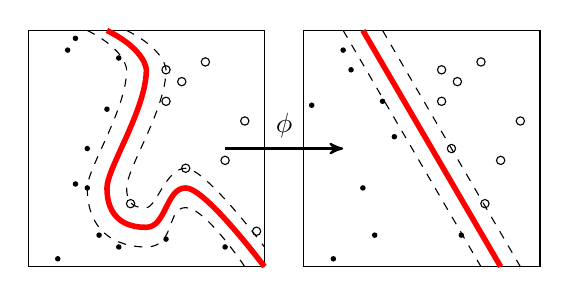
\begin{tikzpicture}[>=stealth',x=1cm,y=1cm, scale = .5]
 
                        %draw[color=gray] (0,0) grid (6,6);
                        \draw (0,0) rectangle (6,6);
                        % \draw line
                        \draw[color=red,line width=2pt]
                          (2,6) .. controls (3,5.5) and (3,5) .. 
                          (3,5) .. controls (3,4) and (2,2.5) .. 
                          (2,2) .. controls (2,1) and (2.8,1) .. 
                          (3,1) .. controls (3.5,1) and (3.5,2) .. 
                          (4,2) .. controls (4.5,2) and (6,0) .. 
                          (6,0);
                        % \draw left dashed line
                        \draw[dashed] 
                          (1.5,6) .. controls (2.5,5.5) and (2.5,5) .. 
                          (2.5,5) .. controls (2.5,4) and (1.5,2.5) .. 
                          (1.5,2) .. controls (1.5,.5) and (2.8,.5) .. 
                          (3,.5) .. controls (3.75,.5) and (3.5,1.5) .. 
                          (4,1.5) .. controls (4.5,1.5) and (5.5,0) .. 
                          (5.5,0);
                        % \draw right dashed line
                        \draw[dashed] 
                          (2.5,6) .. controls (3.5,5.5) and (3.5,5) .. 
                          (3.5,5) .. controls (3.5,4) and (2.5,2.5) .. 
                          (2.5,2) .. controls (2.5,1.5) and (2.8,1.5) .. 
                          (3,1.5) .. controls (3.25,1.5) and (3.5,2.5) .. 
                          (4,2.5) .. controls (4.5,2.5) and (6,0.5) .. 
                          (6,0.5);
                        %\draw[color=gray] (2,6) -- (3,5) -- (2,2) -- (3,1) -- (4,2) -- (6,0);
                        %\draw[color=gray] (1.5,6) -- (2.5,5) -- (1.5,2) -- (3,.5)-- (4,1.5)-- (5.5,0);
                        %\draw[color=gray] (2.5,6) -- (3.5,5) -- (2.5,2) -- (3,1.5)-- (4,2.5)-- (6,0.5);
                         
                        %\draw[color=gray] (7,0) grid (13,6);
                        \draw (7,0) rectangle (13,6);
                        % \draw line
                        \draw[color=red,line width=2pt] (8.5,6) -- (12,0);
                        % \draw dashed line
                        \draw[dashed]  (8,6) -- (11.5,0);
                        \draw[dashed]  (9,6) -- (12.5,0);
                         
                        \draw[->,thick] (5,3) -- (8,3) node [above,pos=.5] {$\phi$};
                         
                        \def\positive{{%
                        {2.3,5.3},
                        {3.5,.7},
                        {1.5,2},
                        {1.2,2.1},
                        {1.8,.8},
                        {1,5.5},
                        {1.2,5.8},
                        {.75,.2},
                        {2,4},
                        {5, 0.5},
                        {1.5,3},
                        {2.3,.5},
                        %
                        {9.3,3.3},
                        {11,.8},
                        {8.5,2},
                        {7.2,4.1},
                        {8.8,.8},
                        {8,5.5},
                        {8.2,5},
                        {7.75,.2},
                        {9,4.2},
                        {12, 0.5},
                        {8.5,3},
                        {9.3,.5},
                        }}
                         
                        % \draw positive dots
                        \foreach \i in {0,...,20} {
                          \pgfmathparse{\positive[\i][0]}\let \x \pgfmathresult;
                          \pgfmathparse{\positive[\i][1]}\let \y \pgfmathresult;
                          \fill[black] (\x,\y) circle (2pt);
                        }
                         
                        \def\negative{{%
                        {4,2.5},
                        {3.5,5},
                        {2.6,1.6},
                        {4.5,5.2},
                        {5.5,3.7},
                        {3.9,4.7},
                        {5,2.7},
                        {3.5,4.2},
                        {5.8,.9},
                        %
                        {10.75,3},
                        {10.5,5},
                        {11.6,1.6},
                        {11.5,5.2},
                        {12.5,3.7},
                        {10.9,4.7},
                        {12,2.7},
                        {10.5,4.2},
                        {12.8,.9},
                        }}
                         
                        % \draw negative dots
                        \foreach \i in {0,...,16} {
                          \pgfmathparse{\negative[\i][0]}\let \x \pgfmathresult;
                          \pgfmathparse{\negative[\i][1]}\let \y \pgfmathresult;
                          \draw[black] (\x,\y) circle (3pt);
                        }
                         
                        \end{tikzpicture}
                    }
        		\end{center}
     \end{column}
 \end{columns}
}

%\subsection{Further Outlook}


\subsection{Practical hints}
\frame{\frametitle{Practical hints for application of data science methods}
\framesubtitle{}
\begin{columns}[t] 
     \begin{column}[T]{6cm} 
     	\begin{itemize}
     		\item Get to know your data
		\item Use training and validation sets
		\item For clustering and ML: 
		\begin{itemize}
		\item Regularise
		\item Remove outliers, NaN
		\end{itemize} 
		\item When building models:
		\begin{itemize}
		\item Don't expect perfect fit
		\item Inspect confusion matrix
		\end{itemize}
     	\end{itemize}
     \end{column}
     	\begin{column}[T]{6cm} 
         	\begin{center}
            		\renewcommand\arraystretch{1.5}
                            \setlength\tabcolsep{0pt}
                            \begin{tabular}{c >{\bfseries}r @{\hspace{0.7em}}c @{\hspace{0.4em}}c @{\hspace{0.7em}}l}
                              \multirow{10}{*}{\parbox{1.1cm}{\bfseries\raggedleft actual\\ value}} & 
                                & \multicolumn{2}{c}{\bfseries Prediction outcome} & \\
                              & & \bfseries p & \bfseries n & \bfseries total \\
                              & p$'$ & \MyBox{True}{Positive} & \MyBox{False}{Negative} & P$'$ \\[2.4em]
                              & n$'$ & \MyBox{False}{Positive} & \MyBox{True}{Negative} & N$'$ \\
                              & total & P & N &
                            \end{tabular}        		
                            \end{center}
     \end{column}
 \end{columns}
}

\frame{\frametitle{Get to work!}
\framesubtitle{Load and try \texttt{2-SVM-and-KMeans.ipynb} }
\begin{center}

\includegraphics[width = .3\textwidth]{Wagenmeister.png}
\end{center}
}




\end{document}
